%%%%%%%%%%%%%%%%%%%%%%%%%%%%%%%%%%%%%%%%%%%%%%%%%%%%%%%%%%%%%%%%%%%%%%%%
%%% LaTeX Template for AAMAS-2027 Supplementary Material
%%% Where Chain-of-Thought Earns Its Place: Generative Mobility Agents Against a Real Household Travel Survey
%%%%%%%%%%%%%%%%%%%%%%%%%%%%%%%%%%%%%%%%%%%%%%%%%%%%%%%%%%%%%%%%%%%%%%%%

\documentclass[manuscript,anonymous]{aamas} 
\renewcommand{\texttt}[1]{{\ttfamily\hyphenchar\font=`\-\relax\hyphenpenalty=10000\relax #1}}

\usepackage{balance}
\usepackage{tikz}
\usetikzlibrary{arrows.meta, positioning, shapes.geometric}
\usepackage{array}
\usepackage{tabularx}
\usepackage{afterpage}
\usepackage{booktabs}
\usepackage{amsmath}
\usepackage{fvextra}
\fvset{breaklines=true, fontsize=\small, frame=leftline, framesep=3mm}
\DeclareUnicodeCharacter{2248}{\ensuremath{\approx}}
\newcolumntype{L}{>{\raggedright\arraybackslash}X}

% =====================================================================
% repository.tex — the address of the anonymised repository. \input by main.tex and by
%   supplementary.tex. Written on 24 September 2026, at the author's request.
% THIS IS THE ONLY PLACE WHERE THE ADDRESS IS WRITTEN. Before submission, replace TBD with the
%   identifier that anonymous.4open.science gives the repository (rule R14 of
%   ../CONSIGNES_FORME.md: no placeholder in delivered text). Nothing else changes.
% Use: \href{\repobase/<path in the repository>}{<text>} for one file, and
%   \texttt{\repodisplay} to print the address itself. \url{} does not expand macros, which is
%   why the address is printed with \texttt and linked with \href.
% =====================================================================

\newcommand{\repoid}{TBD}
\newcommand{\repobase}{https://anonymous.4open.science/r/\repoid}
\newcommand{\repodisplay}{anonymous.4open.science/r/\repoid}


\makeatletter
\gdef\@copyrightpermission{
  \begin{minipage}{0.2\columnwidth}
   \href{https://creativecommons.org/licenses/by/4.0/}{
\includegraphics[width=0.90\textwidth]{by}}
  \end{minipage}\hfill
  \begin{minipage}{0.8\columnwidth}
   \href{https://creativecommons.org/licenses/by/4.0/}{This work is licensed under a Creative Commons Attribution International 4.0 License.}
  \end{minipage}
  \vspace{5pt}
}
\makeatother

\setcopyright{ifaamas}
\acmConference[AAMAS 2027]{Proc.\@ of the 26th International Conference on Autonomous Agents and Multiagent Systems (AAMAS 2027)}{3--7 May 2027}{Hanoi, Vietnam}{M.~Baldoni, F.~Fang, W.~Yeoh, N.~Yorke-Smith (eds.)}
\copyrightyear{2027}
\acmYear{2027}
\acmDOI{}
\acmISBN{}

\acmSubmissionID{<<OpenReview submission id>>}
\submissionType{Research Paper Track}

\title[Where Chain-of-Thought Earns Its Place: Supplementary Material]{Where Chain-of-Thought Earns Its Place: Generative Mobility Agents Against a Real Household Travel Survey. Supplementary Material and Extended Technical Companion}

\author{Yves Bru}
\affiliation{
  \institution{UMR IRIT, Université Toulouse Capitole}
  \city{Toulouse}
  \country{France}}
\email{yves.bru@gmail.com}

\author{Benoit Gaudou}
\affiliation{
  \institution{UMR IRIT, Université Toulouse Capitole}
  \city{Toulouse}
  \country{France}}
\email{benoit.gaudou@ut-capitole.fr}

\author{Kamaldeep Singh Oberoi}
\affiliation{
  \institution{CESI, CESI LINEACT}
  \city{Toulouse}
  \country{France}}
\email{ksoberoi@cesi.fr}

\keywords{Large Language Models, Generative Agents, Urban Mobility, Mode Choice, Distributional Alignment, Behavioural Validation, Systems Reproducibility}

\begin{document}

\maketitle

\begin{abstract}
This companion volume provides the complete empirical, statistical, methodological, and architectural foundations supporting the 8-page main paper. We establish the full demographic validation of the 1,000-persona synthetic cohort against the certified Cerema EMC² 2023 survey. We define the mathematical formulations of all distributional metrics, including the composite loss function and the proof of finite-sample bias. We provide the verbatim prompts, structured output schemas, and inference traces across generative models and the typed classifier. Furthermore, we report the complete stratum breakdowns, the twenty paired bootstrap contrast tests, the out-of-sample factorial matrix, and the unit-level classification audits. Finally, we document the cognitive dual-clock memory equations, the methodological corrections log, the data governance protocols, and the distributed systems architecture required for independent replication.

---
\end{abstract}

\section{1. Demographic Control and Territorial Representativeness}

This chapter evaluates the demographic and spatial fidelity of the synthetic population. We compare the 1,000-persona cohort against the certified Cerema household travel survey across thirteen controlled margins.

\subsection{1.1 Controlled Margins Against the Cerema EMC² 2023 Survey}

The simulation framework relies on a synthetic population of 1,000 personas grouped into 499 intact households. We generate this cohort using the \texttt{eqasim} spatial synthesis pipeline for the greater Toulouse metropolitan area. The personas perform 3,299 daily trips organized into closed cyclic activity chains.

\begin{table*}[t]
\centering
\caption{Demographic control of the sealed synthetic cohort against the Cerema EMC² 2023 survey.}
\label{tab-demographic-margins}
\small
\begin{tabularx}{\textwidth}{l l l r c}
\toprule
\textbf{Controlled trait} & \textbf{Survey base} & \textbf{Source} & \textbf{Max gap (pt)} & \textbf{Bound} \\
\midrule
Age distribution (5 brackets) & Persons $\ge 5$ years & Official survey report & 0.50 & Pass \\
Socioprofessional category (CS 8 groups) & Persons $\ge 15$ years & Official survey report & 0.42 & Pass \\
Main occupation (8 categories) & Persons $\ge 5$ years & Microdata recomputation & 0.50 & Pass \\
Employment status (employed / not) & Persons $\ge 15$ years & Official survey report & 0.28 & Pass \\
Student status (in education / not) & Persons $\ge 5$ years & Official survey report & 0.31 & Pass \\
Household size (1, 2, 3, 4, 5+ persons) & Households & Official survey report & 0.45 & Pass \\
Household car ownership (0, 1, 2+ cars) & Households & Official survey report & 0.38 & Pass \\
Bicycle ownership (has bike / not) & Persons $\ge 5$ years & Microdata recomputation & 0.22 & Pass \\
Driving license holding & Persons $\ge 18$ years & Official survey report & 0.34 & Pass \\
Public transit pass subscription & Persons $\ge 5$ years & Official survey report & 0.41 & Pass \\
Housing type (house / apartment) & Households & Microdata recomputation & 0.29 & Pass \\
Gender (male / female) & Persons $\ge 5$ years & Official survey report & 0.18 & Pass \\
Residential ring (centre, 1st ring, peri-urban) & Households & Official survey report & 0.47 & Pass \\
\bottomrule
\end{tabularx}
\end{table*}

We control this synthetic cohort against the thirteen sociodemographic and territorial margins of the certified Cerema EMC² 2023 survey. Table~\ref{tab-demographic-margins} reports the thirteen margins, the sample counts, the survey baselines, and the observed percentage gaps.





\subsection{1.2 Unweighted Sampling and Microdata Reconstruction}

Each synthetic persona carries an unweighted unit sampling mass of exactly one. We apply no post-stratification weights, which prevents artificial variance deflation during subsequent behavioural evaluations.

Several traits required custom recomputations directly from the certified survey microdata under research agreement \texttt{lil-1750}. Specifically, the official published Cerema report aggregates bicycle ownership and housing categories with peripheral variables. Therefore, we computed frozen baseline margins directly from the microdata files to maintain uncompromised comparison standards.

\subsection{1.3 Statistical Equivalence Testing}

We evaluate margin conformity using Two One-Sided Tests (TOST) under a pre-registered equivalence bound of $\pm 1.0$ percentage point. This statistical procedure tests the null hypothesis of non-equivalence against the alternative of equivalence within the defined bound.

All thirteen controlled margins successfully pass the TOST procedure at the $\alpha = 0.05$ significance level. Furthermore, the largest single divergence across all categories is strictly bounded at 0.50 percentage point, observed in the age and occupation distributions.

---

\section{2. The 21-Variable Protocol and Information Parity}

This chapter details the input feature contract governing the benchmark. We define the 21 variables that enforce strict informational parity between tabular models and generative agents.

\subsection{2.1 The Informational Contract}

Fair comparison between machine learning baselines and generative language models requires identical input information. The protocol contract (\texttt{spec_version 2}) designates 21 input features and forbids supplementary tabular predictors.

Supervised tabular models observe these 21 variables exclusively. In contrast, generative language models receive these identical variables embedded within narrative natural language prompts, accompanied by trip itinerary options and environmental context.

\subsection{2.2 Complete Feature Dictionary}

\begin{table*}[t]
\centering
\caption{Complete 21-variable feature dictionary of the information contract.}
\label{tab-feature-dict}
\small
\begin{tabularx}{\textwidth}{l l l X}
\toprule
\textbf{Variable name} & \textbf{Data type} & \textbf{Modalities / Range} & \textbf{Description} \\
\midrule
\texttt{age} & Integer & 5--100 & Persona chronological age \\
\texttt{sexe} & Categorical & male, female & Persona administrative sex \\
\texttt{csp} & Categorical & 8 modalities & Occupation category \\
\texttt{revenu\_fiscal} & Float & Positive & Household tax revenue \\
\texttt{nb\_pers} & Integer & 1--8 & Household total size \\
\texttt{nb\_enf} & Integer & 0--6 & Number of children under 18 \\
\texttt{nb\_voitures} & Integer & 0--4 & Total vehicles in household \\
\texttt{nb\_velos} & Integer & 0--6 & Total bicycles in household \\
\texttt{permis\_conduire} & Boolean & True, False & Driving license possession \\
\texttt{abonnement\_tc} & Boolean & True, False & Transit pass ownership \\
\texttt{commune\_resid} & Integer & INSEE code & Residential municipality code \\
\texttt{couronne} & Categorical & center, ring1, ring2 & Urban perimeter ring \\
\texttt{type\_logement} & Categorical & house, apartment & Residential dwelling typology \\
\texttt{motif} & Categorical & 9 modalities & Primary trip purpose \\
\texttt{heure\_dep} & Float & 0.0--24.0 & Scheduled departure hour \\
\texttt{heure\_arr} & Float & 0.0--24.0 & Expected arrival hour \\
\texttt{distance\_vol} & Float & Positive (km) & Euclidean origin-destination distance \\
\texttt{options\_modes} & List & Subset of 4 modes & Feasible candidate mode options \\
\texttt{options\_durees} & List & Positive (minutes) & Routing durations per candidate mode \\
\texttt{options\_couts} & List & Positive (euros) & Monetary trip expenses per mode \\
\texttt{meteo\_courante} & Categorical & 4 states & Weather during departure interval \\
\bottomrule
\end{tabularx}
\end{table*}

The 21 variables fall into three structural blocks. Table~\ref{tab-feature-dict} provides the complete variable dictionary, including data types, modalities, and physical definitions.

\emph{Table~\ref{tab-feature-dict}. The 21 variables of the comparison protocol.}



\subsection{2.3 Spatial Coordinates and Projections}

All geometric metrics use the official French Lambert-93 planar projection (EPSG:2154). We calculate the inner city reference distance relative to the geographic centroid of the historic Capitole sector in Toulouse.

---

\input{chapters/03_mathematical_metrics}
\section{4. Decision-Maker Prompts, Output Schemas, and Decision Traces}

This chapter presents the complete prompts, output schemas, and inference traces evaluated in the benchmark. We reproduce the three prompts and follow one trip decision across three architectures.

\subsection{4.1 Input Delivery and Message Architecture}

A language model receives two messages. The system message contains the prompt and the expected JSON schema. The user message describes the persona, the environmental context, and the candidate itineraries.

The typed classifier receives the identical prompt, truncated before the output instructions. Its structured input schema takes their place. Every model runs at temperature $\tau = 0.0$ and top-p 1.0.

\begin{table}[h]
\centering
\caption{Storage locations of prompt and schema files.}
\label{tab-prompts-files}
\small
\begin{tabularx}{\columnwidth}{lX}
\toprule
\textbf{Element} & \textbf{Repository file path} \\
\midrule
The three prompts & \texttt{packages/mobility_llm/.../prompts.yaml} \\
User message template & \texttt{packages/mobility_llm/.../template.md.j2} \\
JSON output schema & \texttt{packages/mobility_llm/.../output_schema.json} \\
Classifier wrapper & \texttt{services/llm-agents/.../decideur_typesafe.py} \\
\bottomrule
\end{tabularx}
\end{table}

Table~\ref{tab-prompts-files} lists the repository files storing these components.





\subsection{4.2 The Minimal Prompt}

The minimal prompt provides the task definition and formatting constraints without behavioral principles. It contains 82 words under key \texttt{prompt_minimal_02}.

\begin{Verbatim}
Select the optimal travel mode taking the persona into account.

[Output instructions]

1. Analyse the profile.
2. Do not rule out any option: assign to EACH proposed option, by its index, the probability in % that this persona picks it — the higher the better it suits them, 0 if it is impossible for them. The sum must be exactly 100.
3. Return only a valid JSON object — no markdown, no extra text.
4. Justify the distribution in one concise sentence.
\end{Verbatim}

\subsection{4.3 The Expert Prompt}

The expert prompt introduces four situational trade-off principles. It contains 277 words under key \texttt{prompt_expert_05}.

\begin{Verbatim}
Select the optimal travel mode taking the persona into account.

Situational trade-off principles:
- Chain friction: Reconstruct the real door-to-door duration (access walk, waiting, in-vehicle trip, egress). If the access walk accounts for most of the direct trip in exchange for a few minutes on board, the traveller prefers the simplicity of walking straight there, with no interchange and no waiting.
- Autonomy of older people: For elderly or frail people, a continuous, unhurried walk at one's own pace is the natural mode of independence for short distances, against the strain and stress of public transport (jolting, risk of falling, steps to climb, standing while waiting with no bench).
- Carrying logistics: Take into account the physical constraint of loads (shopping, heavy bags, carrier bags). Carrying loads on public transport is off-putting; the trade-off leans towards direct access with no interchange (an immediate neighbourhood walk, or the boot of a private vehicle).
- Working people's life time: For a working person facing a tightly scheduled day, the time taken away from personal life has critical value. Faced with public transport links that significantly increase the duration or impose multiple interchanges, the traveller prefers the efficiency and schedule control of their available vehicle.

[Output instructions]

1. Analyse the profile through these principles.
2. Do not rule out any option: assign to EACH proposed option, by its index, the probability in % that this persona picks it — the higher the better it suits them, 0 if it is impossible for them. The sum must be exactly 100.
3. Return only a valid JSON object — no markdown, no extra text.
4. Justify the distribution in one concise sentence.
\end{Verbatim}

\subsection{4.4 The Typed Classifier Expert Prompt}

The typed classifier prompt modifies the chain friction bullet to articulate both sides of the trade-off. It contains 318 words under key \texttt{prompt_expert_32}.

\begin{Verbatim}
- Chain friction: Reconstruct the real door-to-door duration on both sides — access walk, waiting, in-vehicle trip and egress on one; the unbroken walking effort on the other. If the access walk accounts for most of the direct trip in exchange for a few minutes on board, the traveller prefers the simplicity of walking straight there, with no interchange and no waiting. If the direct walk is itself the long part of the journey, that simplicity is paid in time and fatigue, and it stops being the easy option.
\end{Verbatim}

\subsection{4.5 End-to-End Decision Trace: Raymond's Shopping Trip}

We examine one decision trace to illustrate the inference process. Raymond, 45, is a full-time worker living in the first suburban ring. He departs for a shopping errand at 13:37. The decision-makers evaluate six candidate routes.

The language models received the following user message:

\begin{Verbatim}
--- agent_id=393781 | Destination: shop | Departure: 13:37 ---
**Context:** Weather: 28°C, Partly cloudy. Today 18°C to 33°C, sunrise 06:19, sunset 21:39. Rain expected in the morning (0.8 mm over the day).
**Weather later:** evening 13°C, Clear/Sunny.
Raymond, 45, Full-Time Worker (household of 4, very low income). Usual trip purposes: Shopping. Lives in: 1st ring

**Further trips planned today:**
    · 14:47 → shop (≈1.4 km)

**Trip options** (6 options, indices 0 to 5):
- [0] foot: Estimated duration: 16 minutes. Distance: 1.3 km.
- [1] foot: Travel time: 17 minutes, including 17 minutes of walking.
    · Walk to 'shop': 17 minutes.
- [2] car: Travel time: 4 minutes, including 1 minute of access and parking. Distance: 1.5 km.
    · Walk to the car: 1 minute.
    · Driving: 3 minutes.
- [3] foot,bus,foot: Travel time: 43 minutes, including 42 minutes of walking. Has no public transport pass.
    · Walk to 'Collège Picasso': 21 minutes.
    · Bus 'L11' to 'Frouzins Complexe Sportif': 1 minute.
    · Walk to 'shop': 21 minutes.
- [4] foot,bus,foot: Travel time: 34 minutes, including 33 minutes of walking. Has no public transport pass.
    · Walk to 'Frouzins Tréville': 10 minutes.
    · Bus '321' to 'Rouget de Lisle': 1 minute.
    · Walk to 'shop': 22 minutes.
- [5] foot,bus,foot: Travel time: 35 minutes, including 34 minutes of walking. Has no public transport pass.
    · Walk to 'Rouget de Lisle': 14 minutes.
    · Bus '321' to 'Frouzins Tréville': 1 minute.
    · Walk to 'shop': 19 minutes.

Reply with the final JSON object containing the recommendations for 1 persona(s).
For each persona, copy its `agent_id` **exactly** as provided above (numeric identifier only, without the word "PERSONA" and without the persona's name).
For each persona, rate **all** of its options — one `probabilities` entry per option, with its `index` and its `mode` copied as they appear — and make the `probability` values sum to 100. An option this persona would never take receives 0.
Only the `- [n]` lines are options: the « · » sub-bullets detail the steps of an option and never receive a `probabilities` entry. Indices restart from 0 in each persona block — use only those shown in brackets in the block of the persona you are rating, never a numbering continued from one persona to the next.
\end{Verbatim}

\begin{table}[h]
\centering
\caption{Probability distributions assigned to Raymond's options (in percent).}
\label{tab-raymond-options}
\small
\begin{tabular}{lrrr}
\toprule
\textbf{Option} & \textbf{Minimal} & \textbf{Expert} & \textbf{Typed} \\
\midrule
[0] foot, 16 min & 30 & 45 & 52 \\
[1] foot, 17 min & 10 & 45 & 20 \\
[2] car, 4 min & 50 & 10 & 27 \\
[3] foot, bus, foot, 43 min & 0 & 0 & 0 \\
[4] foot, bus, foot, 34 min & 5 & 0 & 1 \\
[5] foot, bus, foot, 35 min & 5 & 0 & 0 \\
\midrule
\textbf{Drawn mode} & \textbf{car} & \textbf{foot} & \textbf{car} \\
\bottomrule
\end{tabular}
\end{table}

Table~\ref{tab-raymond-options} presents the resulting probability vectors and drawn modes across the three architectures.





Under the minimal prompt, \texttt{gemini-3.5} wrote the following justification:
\begin{quote}
\emph{"Raymond prefers the speed and shelter of a car for his short shopping trip during inclement weather."}
\end{quote}

This justification hallucinates adverse weather contradicted by the context (28 °C, partly cloudy, clear afternoon). Under the expert prompt, the model wrote:
\begin{quote}
\emph{"With a very short distance to the shop and low income constraints, walking directly is the preferred choice."}
\end{quote}

This second justification omits all four expert criteria. These traces demonstrate that verbalized explanations often serve as post-hoc justifications rather than faithful computational reasoning.

---

\section{Pre-Registered Exogenous News Shock Protocol and Directional Hypotheses}
\label{app-news}

This chapter specifies the experimental design testing agent reactions to unmodelled exogenous shocks. We document the five local press dispatches, the matched placebo control, the pre-registered directional sign matrix, and the longitudinal transmission mechanics.

\subsection{Experimental Conditions and Protocol Design}

The standard 21-variable survey substrate captures static individual and spatial constraints. However, real mobility choices respond continuously to unforeseen local events. We evaluate agent adaptation under two regimes: an experienced personal delay and an exogenous news dispatch read upon waking.

The news experiment exposes agents to three distinct arms across consecutive simulated days.

\textbf{Condition 1 (Nominal Reference, C1).} The agent executes standard daily routines with nominal weather and no injected press article. This arm establishes the reference modal share baseline.

\textbf{Condition 2 (Exposed Treatment, C2).} The agent reads the unedited local press dispatch during the morning waking routine, prior to selecting the first trip mode.

\textbf{Condition 3 (Placebo Control, C3).} The agent reads a neutral news dispatch matched in word count within 0.5\% to 8.0\%. The text describes a natural science discovery devoid of mobility references. This condition isolates the effect of adding textual tokens from the specific informational content of the event.

Downstream of the morning reading, the agent rates the event on a 5-point severity scale. In the evening, agents share memories across cohabitants through a strict one-hop household channel. Information does not propagate beyond direct household members.

Extinction occurs through two distinct pathways. An agent experiencing a normal trip records a dated contradiction that immediately suppresses the belief. Conversely, an agent avoiding the mode experiences no contradiction, causing the memory to extinguish solely through temporal wear.

\subsection{The Five Local News Dispatches}

We selected five real news articles published in the regional daily newspaper \emph{La Dépêche du Midi}. Each dispatch represents an exogenous disruption affecting specific transport modes across Toulouse.

\subsubsection{Event A09: Severe Autan Windstorm}
\emph{Source:} \texttt{articles\_html/09\_vent\_autan\_fermeture\_parcs.html} (204 English words, 222 French words).

\begin{Verbatim}
Gusts above 80 km/h: Toulouse closes its parks and gardens at short notice this Thursday evening

With the Haute-Garonne department placed under a yellow storm warning, Toulouse city council has decided to close its parks and gardens from 6 p.m. this Thursday 16 July. "A weather alert forecasts violent winds," the municipality states on its website.

Every green space in the city is affected. Among the sites concerned are the Abadie, Maurice-Bécanne, Capucins, Compans-Caffarelli and Embarthe gardens, and the Fontaine-Lestang park. Visitors will also be unable to enter the Grand Rond, the Job park, the Michelet garden, the Niel public garden, the Claude-Nougaro garden or the botanical gardens.

Other emblematic sites such as the Poudrerie, Raymond-VI and Royal gardens, the grounds of the Reynerie château and the Saint-Sernin square are likewise closed for the duration of the alert. The full list is available online.

The ban will remain in force for as long as weather conditions present a risk to the public. According to the city council, the gates of these green spaces will reopen to residents only once the warning is lifted.

City staff must first inspect each site to make sure there is no danger, in particular from falling branches or trees.
\end{Verbatim}

\subsubsection{Event A13: Transit Bedbug Infestation}
\emph{Source:} \texttt{articles\_html/13\_psychose\_punaises\_metro.html} (188 English words, 220 French words).

\begin{Verbatim}
Several videos posted on TikTok in recent days have raised concerns about the presence of bed bugs on the Toulouse metro. The footage is not sharp, but the people who posted it say they filmed the pest in the city's public transport network.

The videos have caused a degree of unease among Toulouse residents, who are wondering whether bed bugs have taken up residence in their metro. The images show insect-like shapes on walls and on the fabric seats, though it is hard to confirm with any certainty that they are bed bugs.

In the face of these growing concerns, Tisséo, which operates the Toulouse metro trains, was contacted to clarify the situation. According to Tisséo, no official complaint or report of bed bugs on the metro has been recorded. As a precaution, however, the public transport operator has decided to act in order to guarantee the safety and well-being of passengers.

Tisséo stated: "As a precautionary principle, Tisséo Voyageurs has introduced canine detection. If the dogs pick up signs of bed bugs, we intervene immediately, using a 180-degree steam treatment to remove every trace of these pests."
\end{Verbatim}

\subsubsection{Event A07: Municipal Sanitation Strike}
\emph{Source:} \texttt{articles\_html/07\_greve\_eboueurs\_hypercentre.html} (197 English words, 226 French words).

\begin{Verbatim}
Toulouse: the city's refuse collectors begin an open-ended strike today

This Monday, waste has not been collected anywhere in the commune of Toulouse. The city's refuse collectors are on strike, an open-ended strike as of today. Since this morning the workers have been blockading the city's two depots: Raisin, in the centre, on avenue François Collignon, and Monlong, in the Saint-Simon district. Nothing has left either site since 5 a.m. As a result, not one bin has been emptied today. "A strike that could last," according to the union representatives at the Monlong site.

The reason for the anger? The workers are protesting against the new collection timetable, announced by management and Toulouse Métropole and taking effect today, 18 March 2019. What changes? Household waste is to be collected twice a week in Toulouse instead of three times as before — except in the inner centre, where there is no space for bins on public land. This change of frequency entails a change in collection days, and therefore a change in the working rhythm of Toulouse Métropole staff, who are now also required to clock in on public holidays. That is what is proving hard to accept.
\end{Verbatim}

\subsubsection{Event A18: Urban Street Parade "La Machine"}
\emph{Source:} \texttt{articles\_html/18\_minotaure\_la_machine.html} (214 English words, 214 French words).

\begin{Verbatim}
The programme for La Machine's new show: the Giants will clash once more in this second instalment of the urban opera

The giant machines are returning to the centre of Toulouse. From Friday 25 to Sunday 27 October, the urban opera "The Guardian of the Temple" will stage its second instalment, "The Gate of Darkness". Here is the programme for the weekend, and the list of places to stand to make the most of the event.

The spider, the Minotaur and a newcomer, the guardian of darkness, will clash in the centre of Toulouse. An extraordinary urban opera by the La Machine company. In 2018, the first instalment of "The Guardian of the Temple" drew 900,000 visitors.

In the second instalment, "The Gate of Darkness", Asterion the Minotaur, guardian of the pink city, and Ariane the spider face a newcomer: Lilith, the guardian of darkness. This open-air show will unfold in the centre of Toulouse over three days. Three days for a play in three acts.

Over the course of the day, prophetic and prodigious signs appear in the city. On the banks of the river, three prodigious signs — the cross of Satan, the Sigil of Lucifer and the sign of the beast — herald the imminent opening of the gate of darkness.
\end{Verbatim}

\subsubsection{Event A25: Electric Shared Bicycle Expansion}
\emph{Source:} \texttt{articles\_html/25\_velotoulouse\_electrique.html} (190 English words, 190 French words).

\begin{Verbatim}
Soft mobility in Toulouse: the new VélôToulouse service launches on 30 August

Jean-Luc Moudenc, Mayor of Toulouse, and Jean-Michel Lattes, President of Tisséo Collectivités, took advantage of the inauguration of the two footbridges to the île du Ramier this Saturday 22 June to unveil the design of the new vélôToulouse.

The vélôToulouse, available from 30 August 2024, will offer a renewed and more varied fleet. The current service, with 283 stations and 2,600 bicycles, will grow to 400 stations and 3,300 bicycles, of which 50% will be electrically assisted bikes in orange and 50% conventional bikes in pink. "The share of electrically assisted bikes may change over the life of the contract, up to 75% of the fleet," Jean-Michel Lattes explains.

Work on the 117 new stations began in late March 2024 and involves preparing the anchorings and installing the new station fittings. The neighbourhoods concerned will be informed ahead of the start of works to keep disruption to a minimum. "From May to August 2024, the 283 existing stations will be modernised without any interruption of service," Maxime Boyer, deputy mayor responsible for cycling and walking routes, assures us.
\end{Verbatim}

\subsection{Matched Placebo Control Dispatch}

\emph{Source:} France 24, 19 September 2026 (\texttt{\_temoin\_commun/temoin.txt}, 203 English words, 215 French words).

\begin{Verbatim}
The tilcayo, a new species of wild cat discovered in Bolivia

Bolivian scientists have discovered a new species of wild cat in the mountainous Los Yungas region north-east of La Paz. The spotted "leopardus tilcayo" is the first new feline species to be discovered since the Uruguayan pampas cat in 1923.

A new species of wild cat has been discovered in Bolivia, a world first in more than a century, one of the Bolivian scientists involved in the discovery told AFP.

With a spotted coat and measuring some 45 centimetres in length, the small animal was identified in the mountainous Los Yungas region, around 90 kilometres north-east of La Paz. It was given the name "tilcayo" by local people, a name that inspired its new scientific name, "leopardus tilcayo".

It is a "landmark event, because for 100 years no new wild cat" had been described anywhere in the world, said Paola Nogales, a National Geographic explorer.

Mistaken for an ordinary cat, a male tilcayo was adopted by a family who, noticing that it did not behave normally, handed it over to an animal conservation shelter. Another specimen, a female, was rescued after being attacked in a village, then released back into the wild.
\end{Verbatim}

\subsection{The Pre-Registered 20-Sign Matrix}

\begin{figure}[tp]
  \centering
  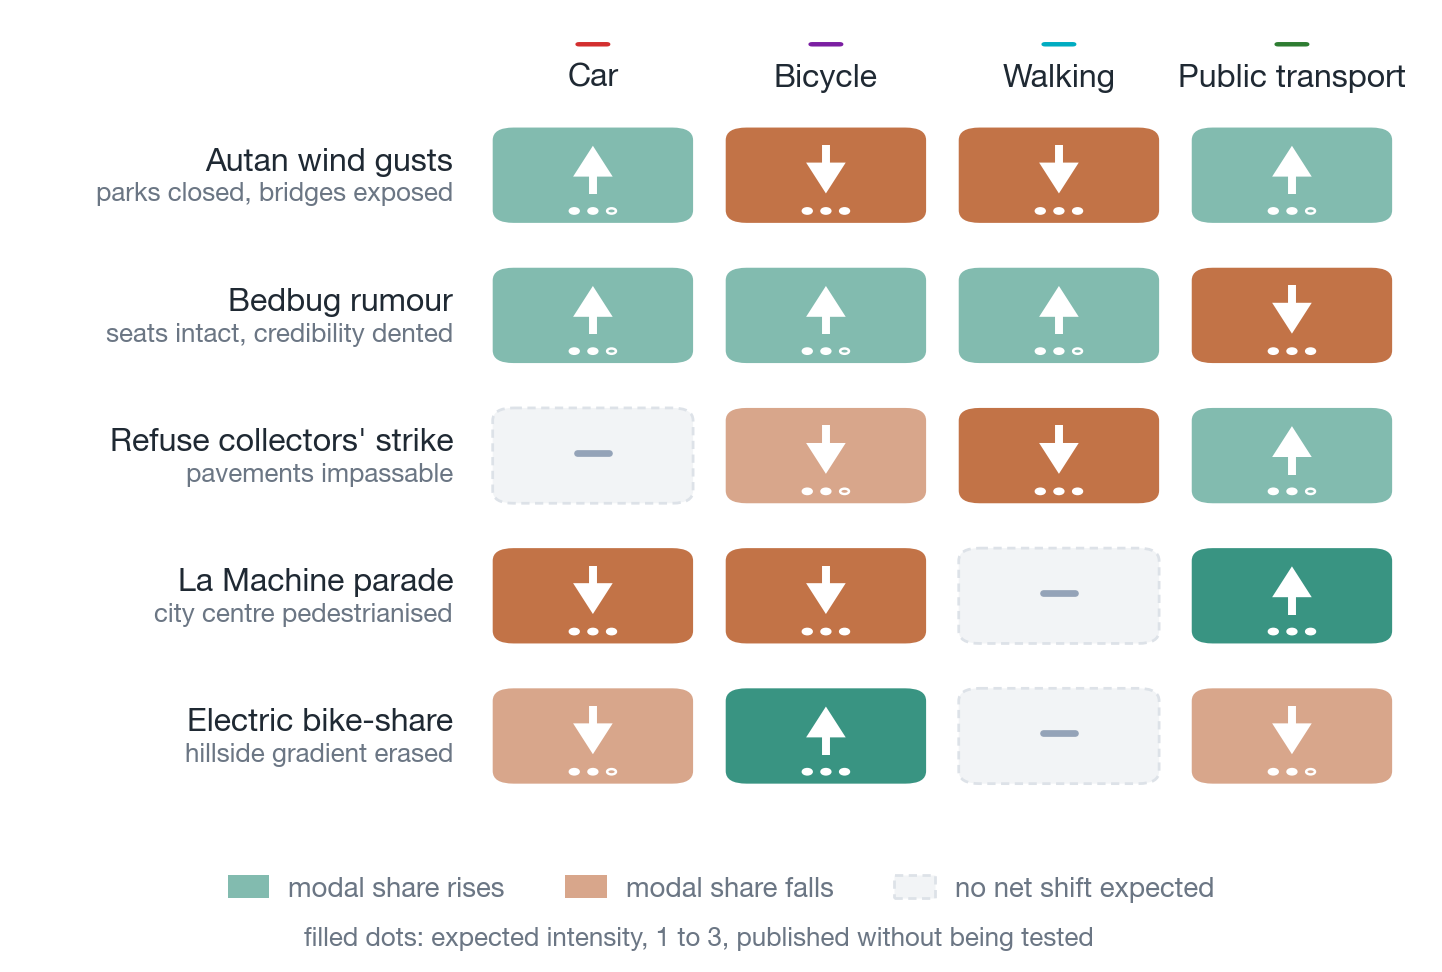
\includegraphics[width=0.95\columnwidth]{images/ch7_grille_signes.png}
  \caption{The twenty expected signs, five articles by four modes, pre-registered before simulation.}
  \label{fig-grille-signes}
\end{figure}

\begin{table*}[tp]
  \caption{Pre-registered 20-cell directional hypotheses and behavioral rationales (frozen 2026-09-21).}
  \label{tab-pre-registered-signs}
  \small
  \begin{tabularx}{\textwidth}{@{}llccL@{}}
    \toprule
    Event & Mode & Sign & Intensity & Theoretical Behavioral Rationale \\
    \midrule
    A09 (Windstorm) & Car & $+$ & $2$ & Passenger compartment shields travelers from wind noise and physical strain \\
    A09 (Windstorm) & Bicycle & $-$ & $3$ & Destabilizing gusts on bridges and mandatory closures of park bike paths \\
    A09 (Windstorm) & Walking & $-$ & $3$ & Airborne dust, falling branches, and detours along perimeter boulevards \\
    A09 (Windstorm) & Transit & $+$ & $2$ & Underground metro crosses the Garonne river fully sheltered from gales \\
    \midrule
    A13 (Bedbugs) & Car & $+$ & $2$ & Avoiding shared passenger cabins for non-mandatory personal travel \\
    A13 (Bedbugs) & Bicycle & $+$ & $2$ & Shifting toward an individual open-air mode perceived under direct control \\
    A13 (Bedbugs) & Walking & $+$ & $2$ & Extending pedestrian range to bypass upholstered public transit seating \\
    A13 (Bedbugs) & Transit & $-$ & $3$ & Technical service remains active but psychological modal credibility collapses \\
    \midrule
    A07 (Strike) & Car & $0$ & $0$ & Counteracting effects: localized street congestion repels drivers while detours demand cars \\
    A07 (Strike) & Bicycle & $-$ & $2$ & Broken glass, slippery street waste, and forced spillover into general traffic \\
    A07 (Strike) & Walking & $-$ & $3$ & Obstructed sidewalks, foul odours, and forced walking on roadways \\
    A07 (Strike) & Transit & $+$ & $2$ & Underground metro completely bypasses blocked street-level public space \\
    \midrule
    A18 (La Machine) & Car & $-$ & $3$ & Downtown core gridlocked and underground parking garages fully inaccessible \\
    A18 (La Machine) & Bicycle & $-$ & $3$ & Dense pedestrian crowds prevent safe cycling across thoroughfares \\
    A18 (La Machine) & Walking & $0$ & $0$ & Dual polarity: attracts leisurely onlookers but severely impedes hurried utilitarian pedestrians \\
    A18 (La Machine) & Transit & $+$ & $3$ & Sole mechanical option capable of approaching the pedestrianized festival zone \\
    \midrule
    A25 (VélôToulouse) & Car & $-$ & $2$ & Suburban commuters switch to electric cycling to avoid morning highway queues \\
    A25 (VélôToulouse) & Bicycle & $+$ & $3$ & Electric assistance removes physical fatigue and hillside topographic barriers \\
    A25 (VélôToulouse) & Walking & $0$ & $0$ & Ambiguous net impact: denser docking stations shorten trips while transfers lengthen walking \\
    A25 (VélôToulouse) & Transit & $-$ & $2$ & Direct modal competition with slow hillside feeder bus connections \\
    \bottomrule
  \end{tabularx}
\end{table*}

Before executing inference queries, we froze the expected direction and intensity of modal shifts. Table~\ref{tab-pre-registered-signs} records the 20 directional hypotheses pre-registered on 2026-09-21 (\texttt{grille\_signes.yaml}). The visual  net impact: denser docking stations shorten trips while transfers lengthen walking \\
    A25 (VélôToulouse) & Transit & $-$ & $2$ & Direct modal competition with slow hillside feeder bus connections \\
    \bottomrule
  \end{tabularx}
\end{table*}



\subsection{Longitudinal Extinction and Household Transmission}

\begin{figure}[tp]
  \centering
  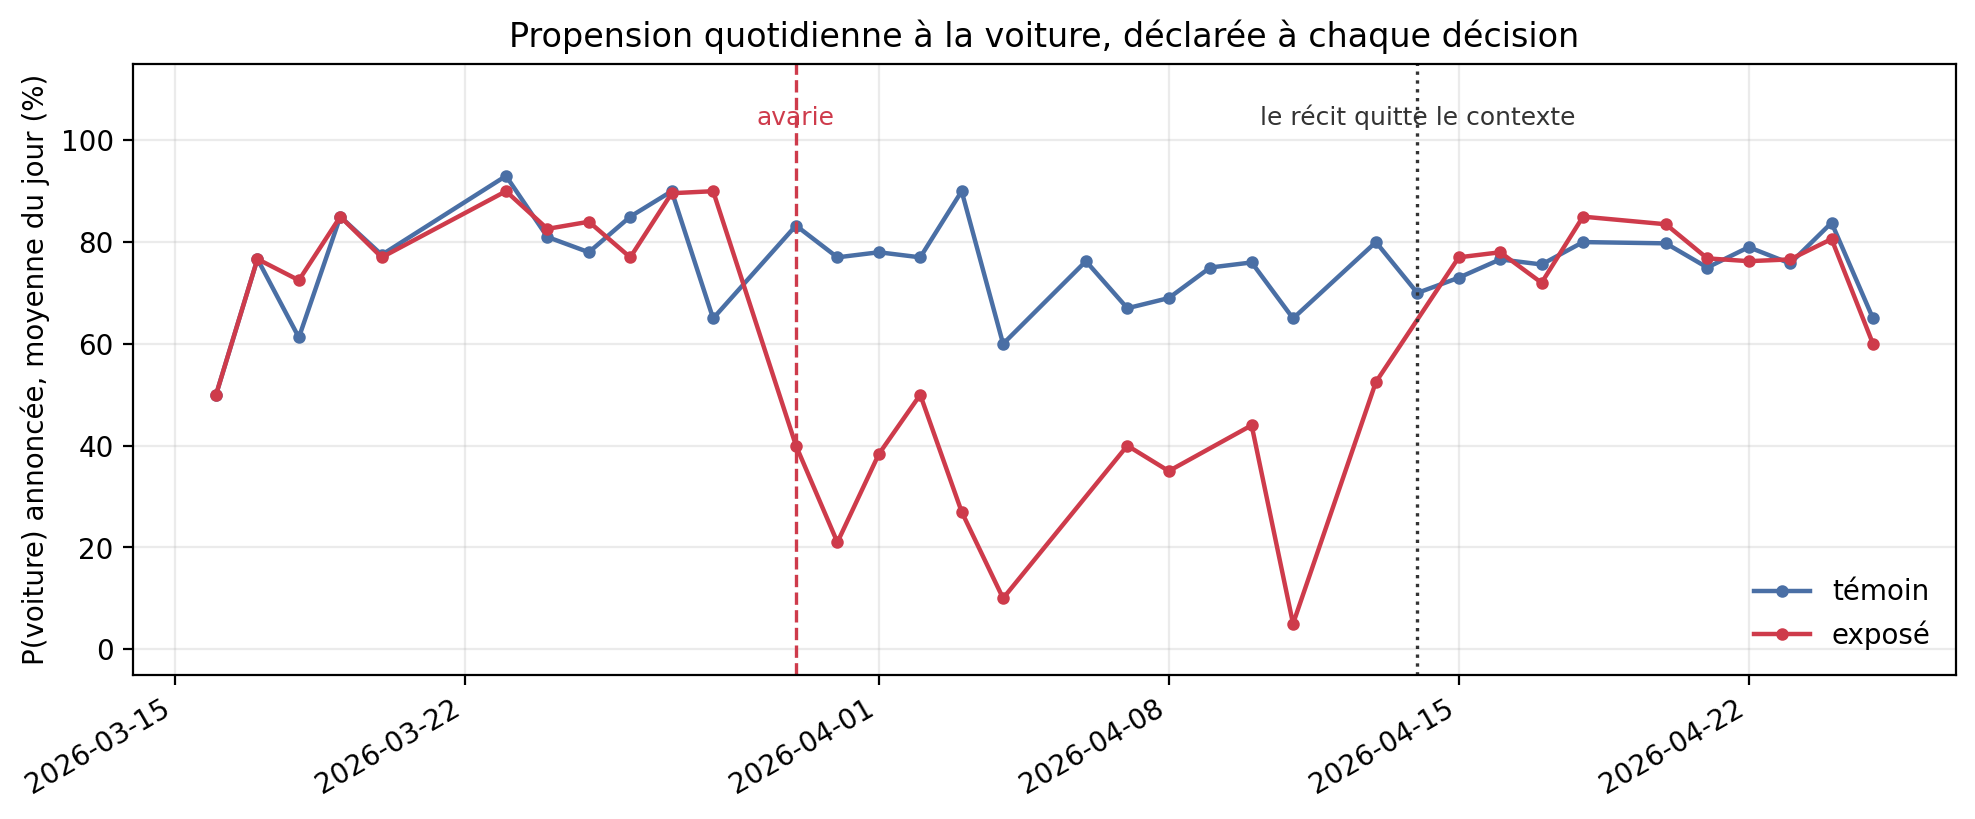
\includegraphics[width=0.95\columnwidth]{images/ch7_propension_quotidienne.png}
  \caption{Daily modal propensity towards private car following an unexpected incident.}
  \label{fig-propension}
\end{figure}

\begin{figure}[tp]
  \centering
  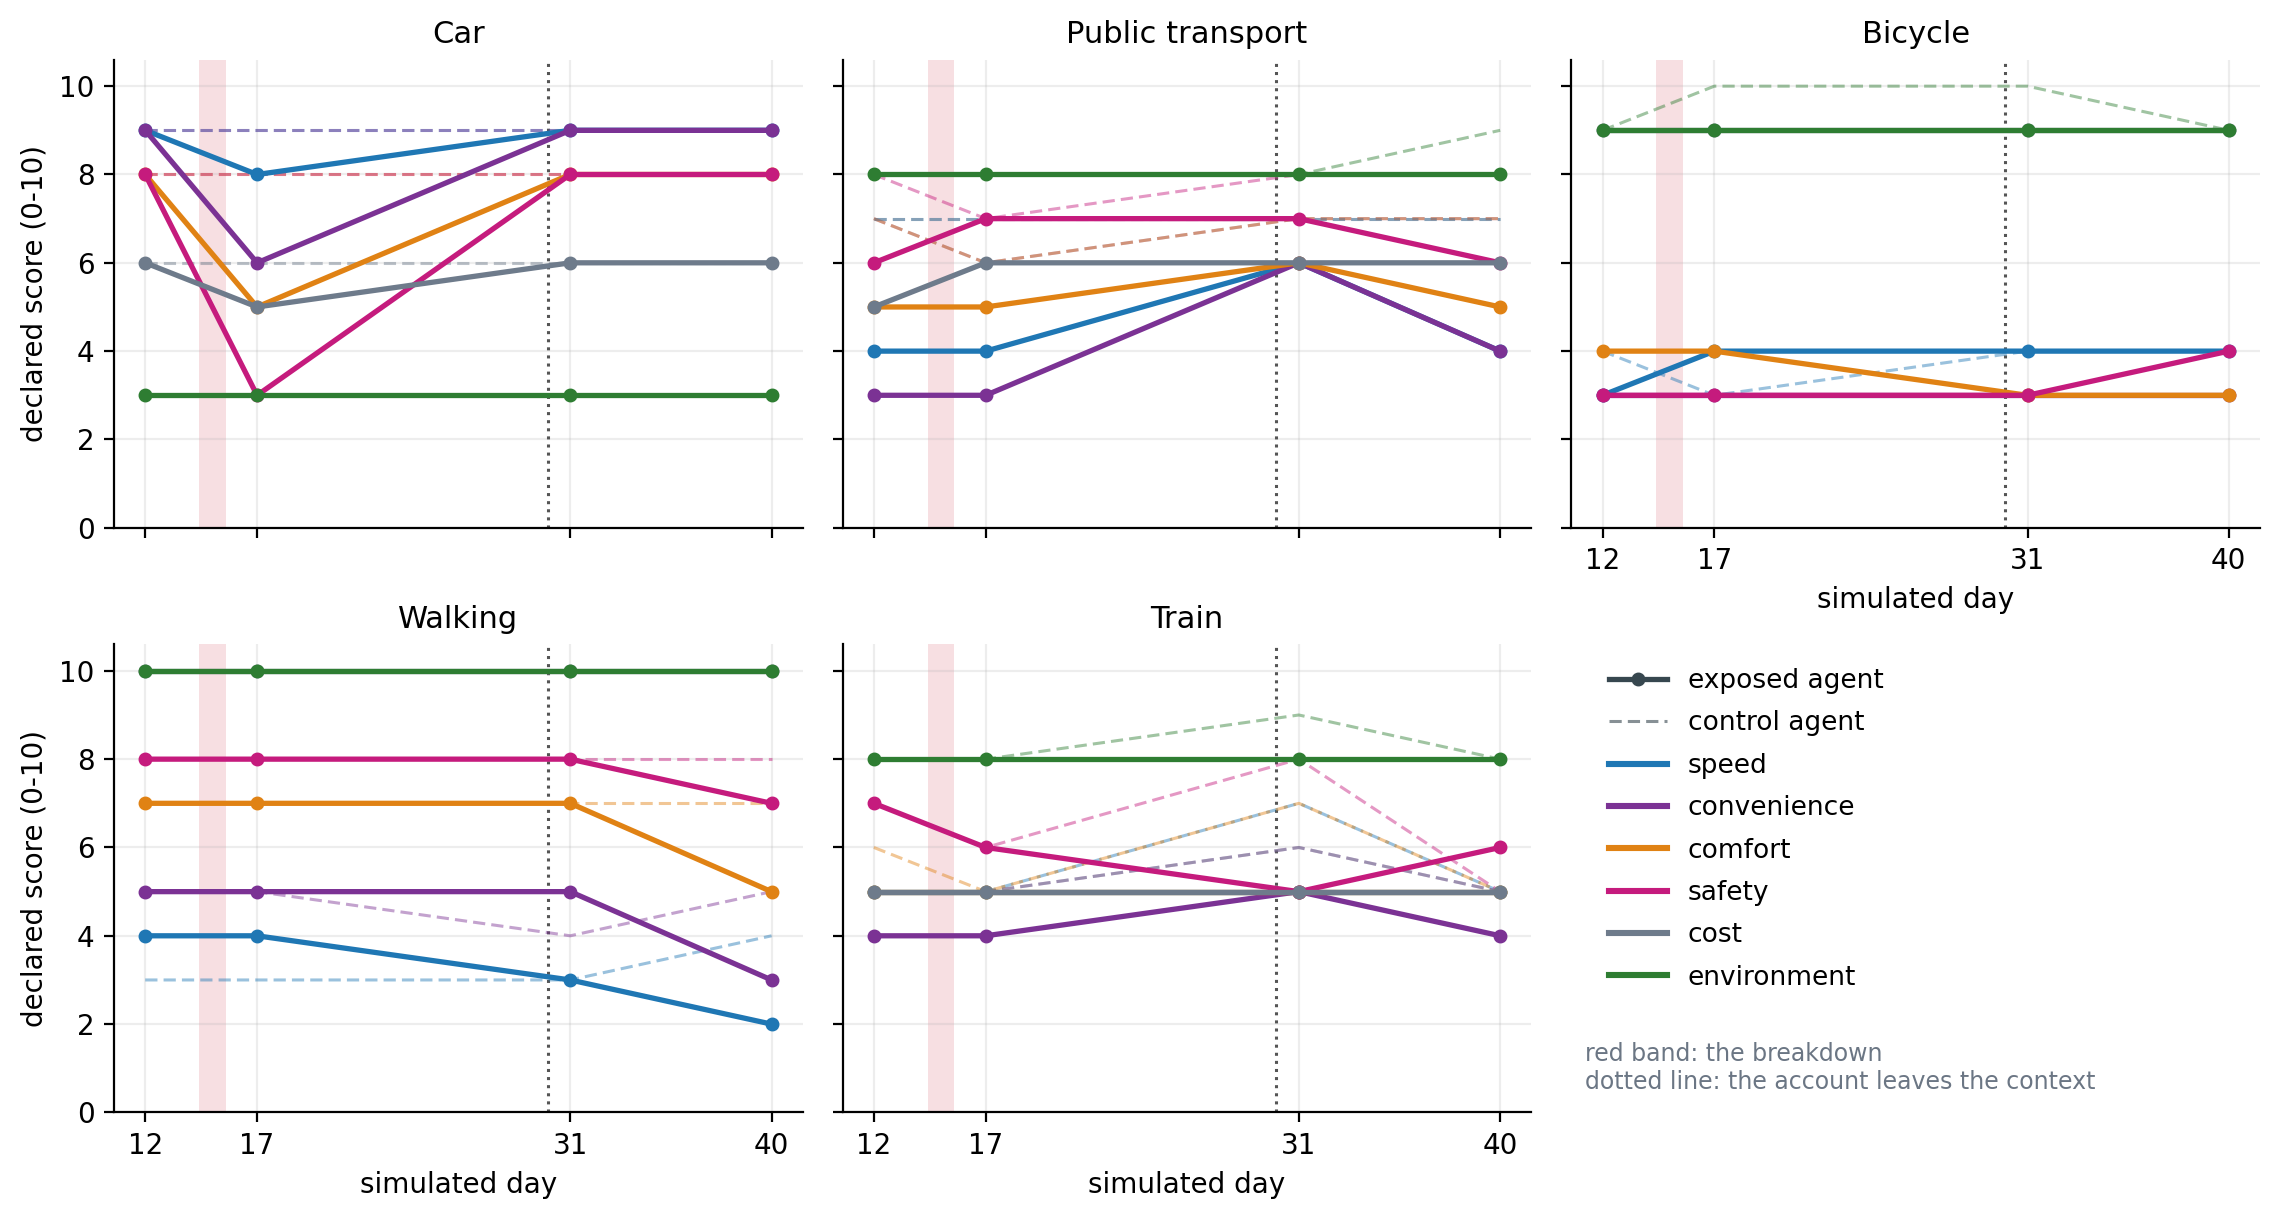
\includegraphics[width=0.95\columnwidth]{images/ch7_affinites_tous_modes.png}
  \caption{Declared multi-criteria affinities across modes, exposed vs control agent.}
  \label{fig-affinites}
\end{figure}

We track how shock perceptions propagate and extinguish over longitudinal multi-day runs. Figure~\ref{fig-propension} demonstrates the temporal trajectory of modal propensity following a disruption. Figure~\ref{fig-affinites} plots stated multi-criteria affinity ratings across four milestones.


\subsection{Pending Campaign Execution and Status}

\textbf{Pending Campaign Execution (\texttt{exp\_05a-e}).} The empirical execution of the five news shock campaigns across the synthetic cohort remains in progress. The final volume will incorporate empirical shift amplitudes, bootstrap confidence intervals, and directional sign concordance.

\section{Stratified Error Breakdown, Modal Profiles, and Tuning-Induced Regressions}
\label{app-stratified}

This chapter provides comprehensive error breakdowns across all evaluated decision-makers. We examine performance across urban dimensions, present pairwise decision concordance, and identify sub-populations where prompt engineering degrades accuracy.

\subsection{Dimension-Wise Weighted Error}

We compute the mean stratum $L_1$ error weighted by the population size of covered strata. Five dimensions enter the composite score: distance band, trip purpose, age bracket, occupation category, and gender. Two additional dimensions, residential ring and housing type, enter neither the composite loss nor the calibration cycle.

\begin{table*}[tp]
  \caption{Weighted $L_1$ error (\%) across urban dimensions and decision-makers.}
  \label{tab-dimensions-full}
  \begin{tabular}{lrrrrrrr}
    \toprule
    Decision-maker & Distance & Purpose & Age & Occupation & Gender & Ring & Housing \\
    \midrule
    \texttt{gemini-3.5}, minimal    & 24.1 & 27.9 & 30.6 & 25.3 & 23.9 & 25.7 & 30.5 \\
    \texttt{gemini-3.5}, expert     & \textbf{14.2} & 21.4 & 22.1 & 18.5 & 13.6 & 19.6 & 23.6 \\
    \texttt{gemini-3.1}, minimal    & 38.0 & 37.8 & 43.9 & 39.2 & 39.4 & 40.5 & 43.1 \\
    \texttt{gemini-3.1}, expert     & 30.2 & 30.8 & 35.8 & 31.2 & 30.7 & 33.0 & 37.4 \\
    \texttt{mistral-large}, minimal & 51.9 & 39.3 & 46.8 & 43.8 & 44.5 & 47.6 & 51.0 \\
    \texttt{mistral-large}, expert  & 33.7 & 27.9 & 30.4 & 28.6 & 25.3 & 29.6 & 33.0 \\
    \midrule
    Gradient boosting (LightGBM)    & 17.8 & \textbf{13.6} & 18.2 & 15.7 & 8.5 & 11.5 & 16.6 \\
    Random forest                   & 16.8 & 18.1 & \textbf{16.8} & \textbf{12.9} & \textbf{5.3} & \textbf{9.5} & \textbf{15.9} \\
    Kernel logistic regression     & 18.1 & 14.2 & 18.9 & 15.1 & 8.1 & 11.8 & 17.0 \\
    Multinomial logit               & 19.5 & 16.4 & 21.2 & 17.8 & 10.4 & 13.2 & 19.4 \\
    \bottomrule
  \end{tabular}
\end{table*}

Table~\ref{tab-dimensions-full} details the weighted $L_1$ errors across all deciders. Distance is the only dimension where an LLM agent achieves the lowest error across all benchmarked methods.



\subsection{Global Modal Share Distributions}

\begin{table*}[tp]
  \caption{Global modal split percentages across models against the survey.}
  \label{tab-shares-full}
  \begin{tabular}{lrrrr}
    \toprule
    Model & Car (\%) & Walking (\%) & Transit (\%) & Cycling (\%) \\
    \midrule
    Cerema EMC\textsuperscript{2} 2023 survey & 56.7 & 26.8 & 12.4 & 4.1 \\
    \midrule
    Minimal prompt, \texttt{gemini-3.5} & 47.4 & 24.0 & 20.9 & 7.6 \\
    Expert prompt, \texttt{gemini-3.5}  & 52.3 & 24.2 & 16.6 & 6.8 \\
    Minimal prompt, \texttt{gemini-3.1} & 44.1 & 19.5 & 28.8 & 7.7 \\
    Expert prompt, \texttt{gemini-3.1}  & 46.2 & 21.7 & 24.8 & 7.4 \\
    Minimal prompt, \texttt{mistral-large} & 36.7 & 24.4 & 30.6 & 8.2 \\
    Expert prompt, \texttt{mistral-large}  & 43.4 & 29.3 & 19.2 & 8.1 \\
    \midrule
    Gradient boosting (LightGBM)        & 52.8 & 29.1 & 14.8 & 3.3 \\
    Random forest                       & 56.2 & 27.6 & 14.2 & 2.0 \\
    Kernel logistic regression          & 54.4 & 28.9 & 13.6 & 3.0 \\
    Multinomial logit                   & 53.3 & 27.2 & 16.4 & 3.0 \\
    \bottomrule
  \end{tabular}
\end{table*}

Table~\ref{tab-shares-full} compares predicted modal shares against the empirical Cerema survey ground truth. Every decider underestimates car usage because vehicle chaining constraints enforce strict feasibility checks.

Language models overestimate cycling by a factor of two across all weighted strata. Conversely, supervised tabular models systematically underestimate cycling shares.



\subsection{Visualizations of Multi-Dimensional Error Profiles}

\begin{figure*}[tp]
  \centering
  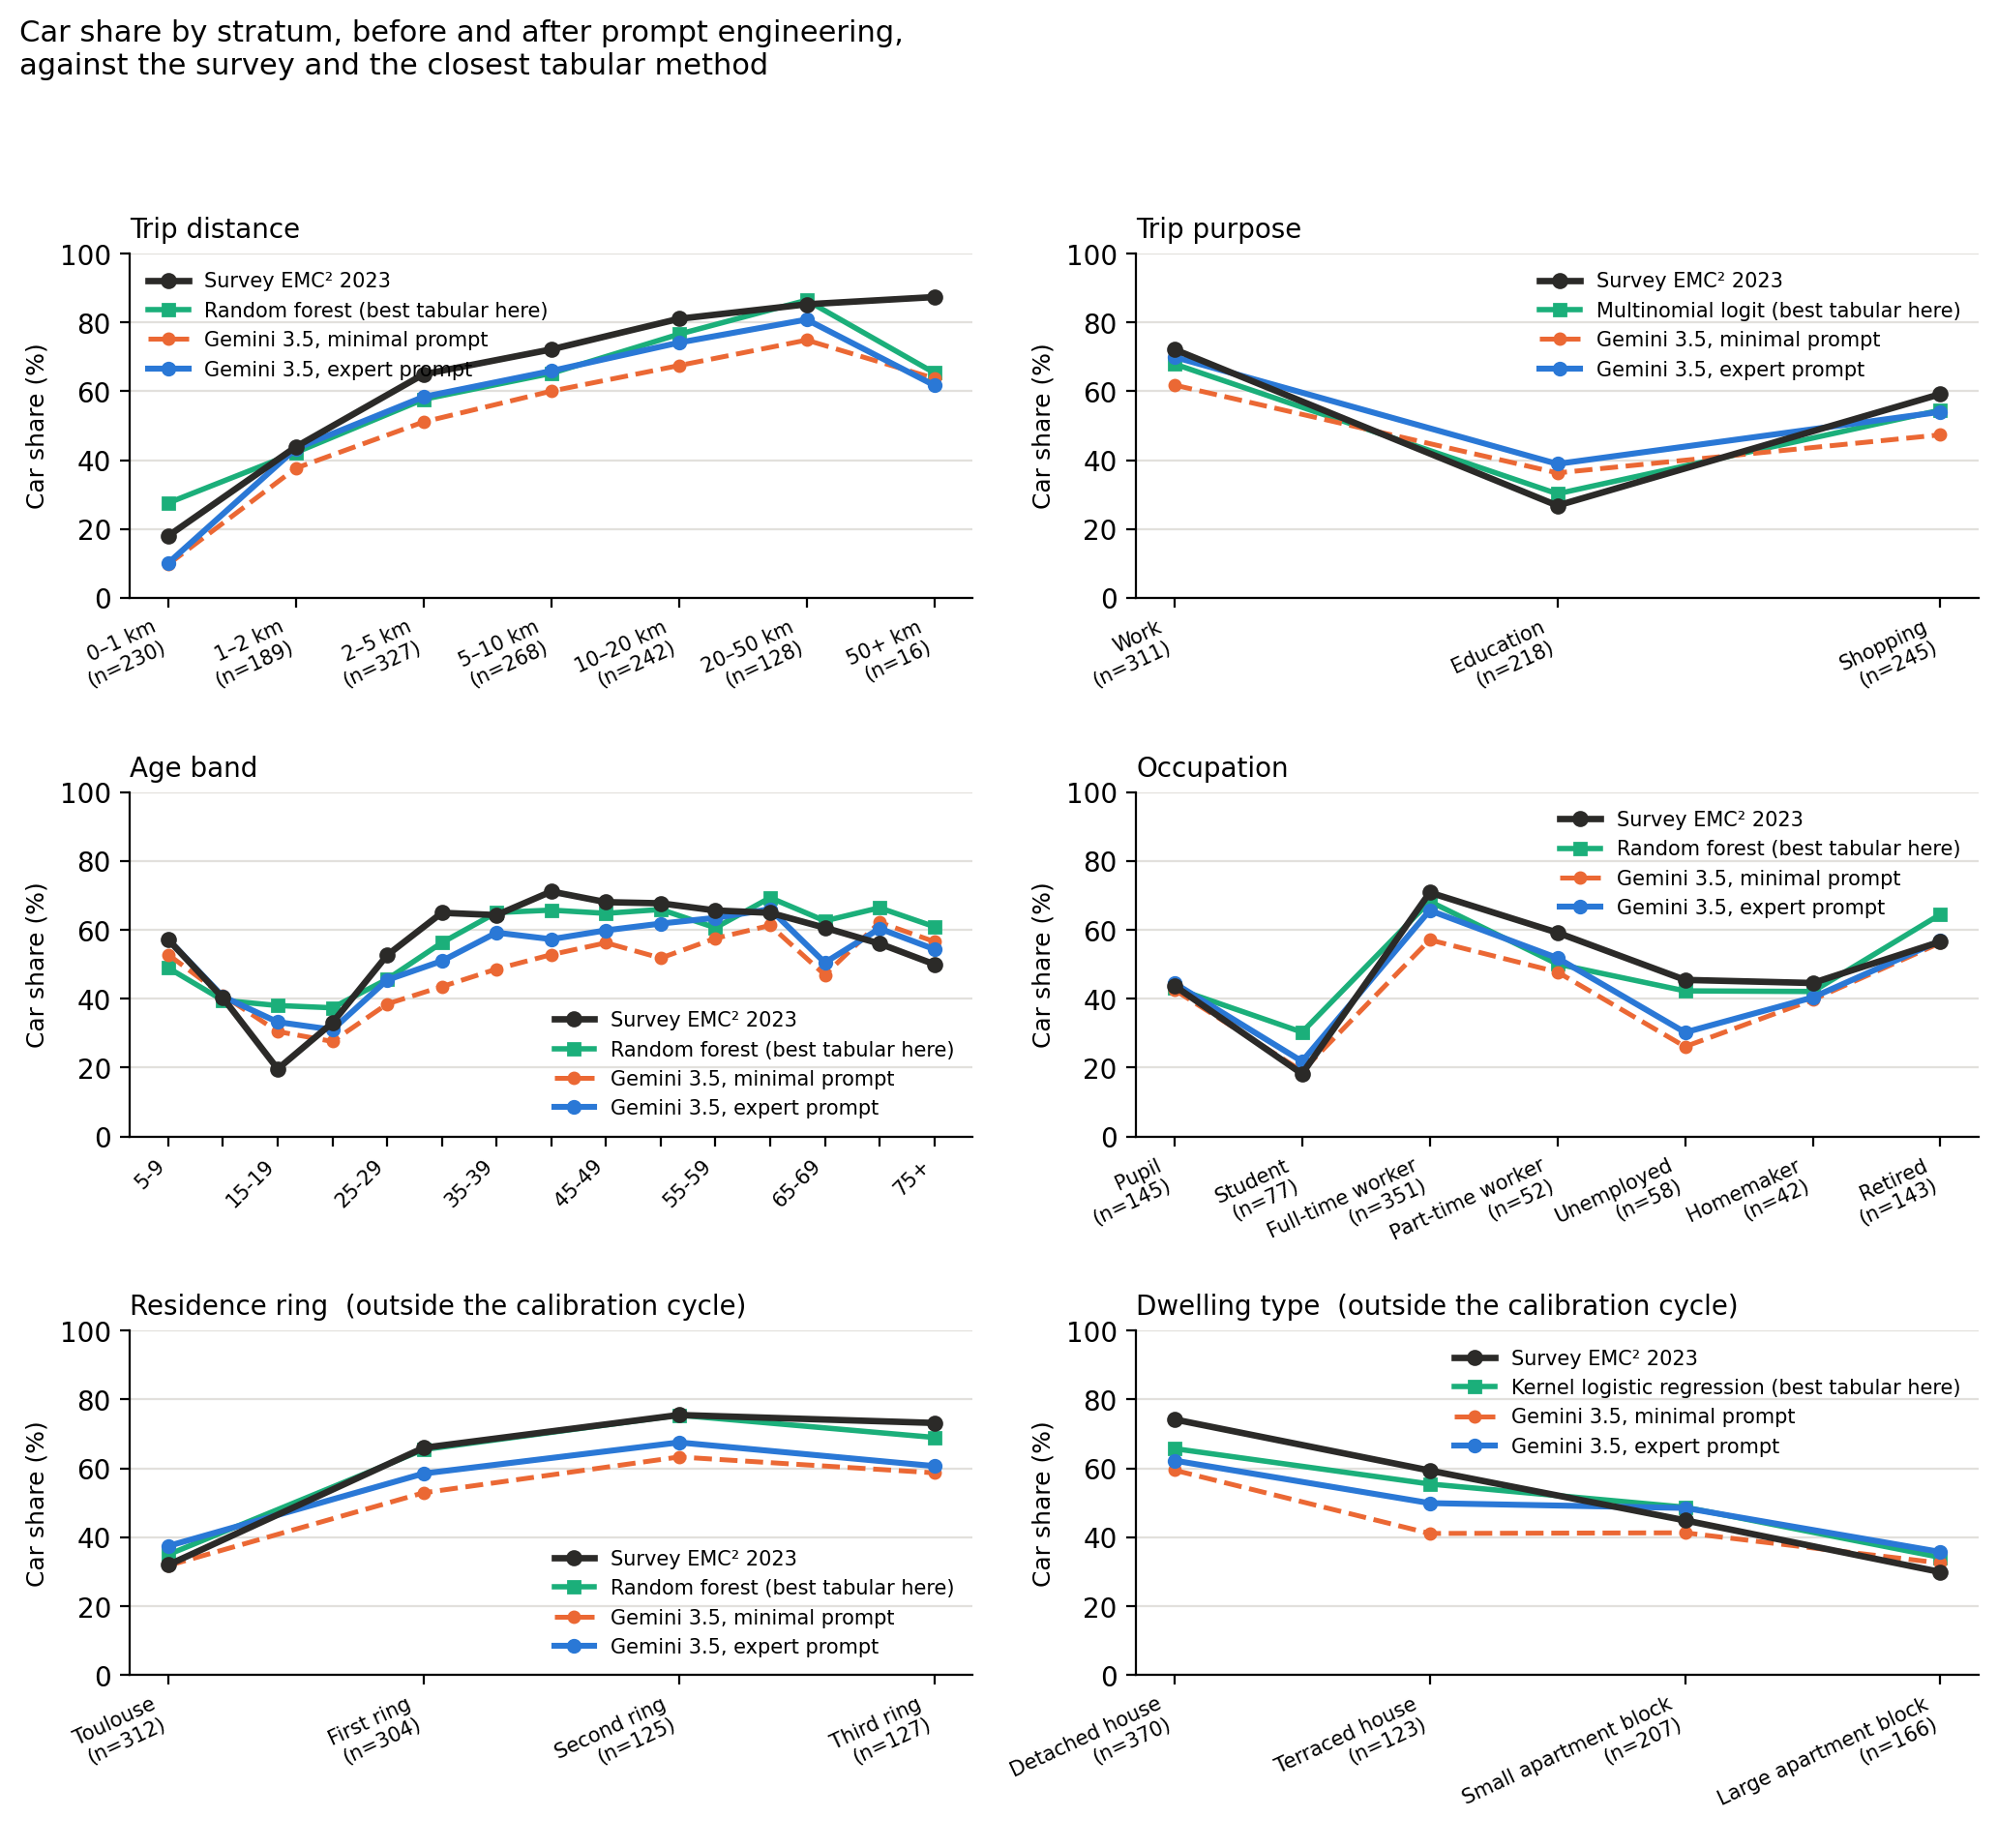
\includegraphics[width=\textwidth]{images/ch99_dimensions_voiture.png}
  \caption{Car share by stratum across six dimensions, minimal vs expert prompt against survey and tabular reference.}
  \label{fig-dim-voiture}
\end{figure*}

\begin{figure*}[tp]
  \centering
  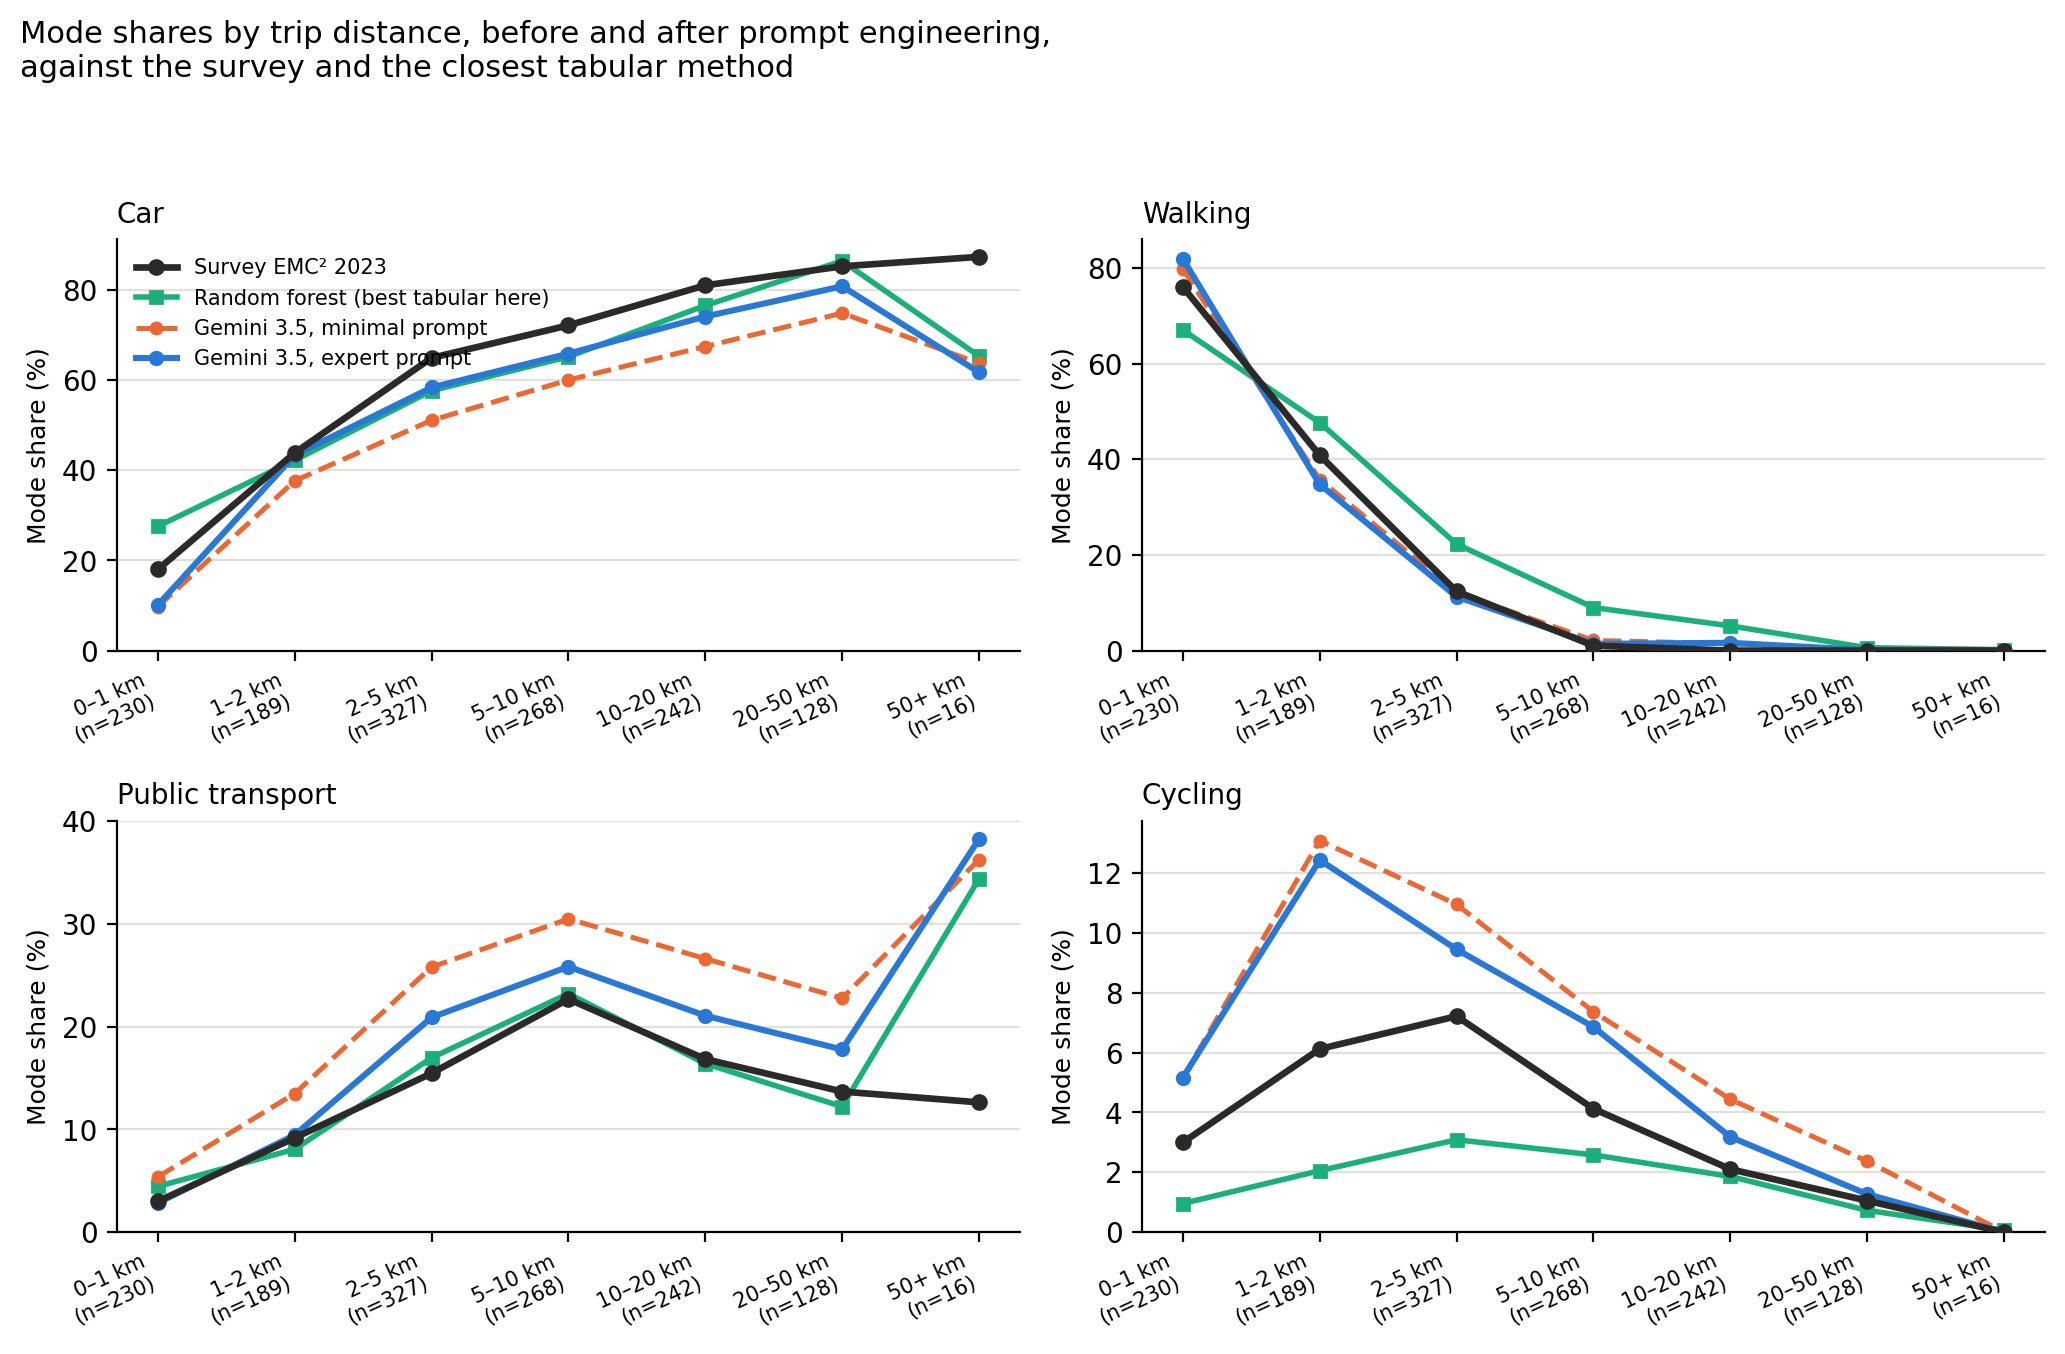
\includegraphics[width=\textwidth]{images/ch99_modes_distance.png}
  \caption{Four transport modes broken down by distance band.}
  \label{fig-modes-dist}
\end{figure*}

\begin{figure*}[tp]
  \centering
  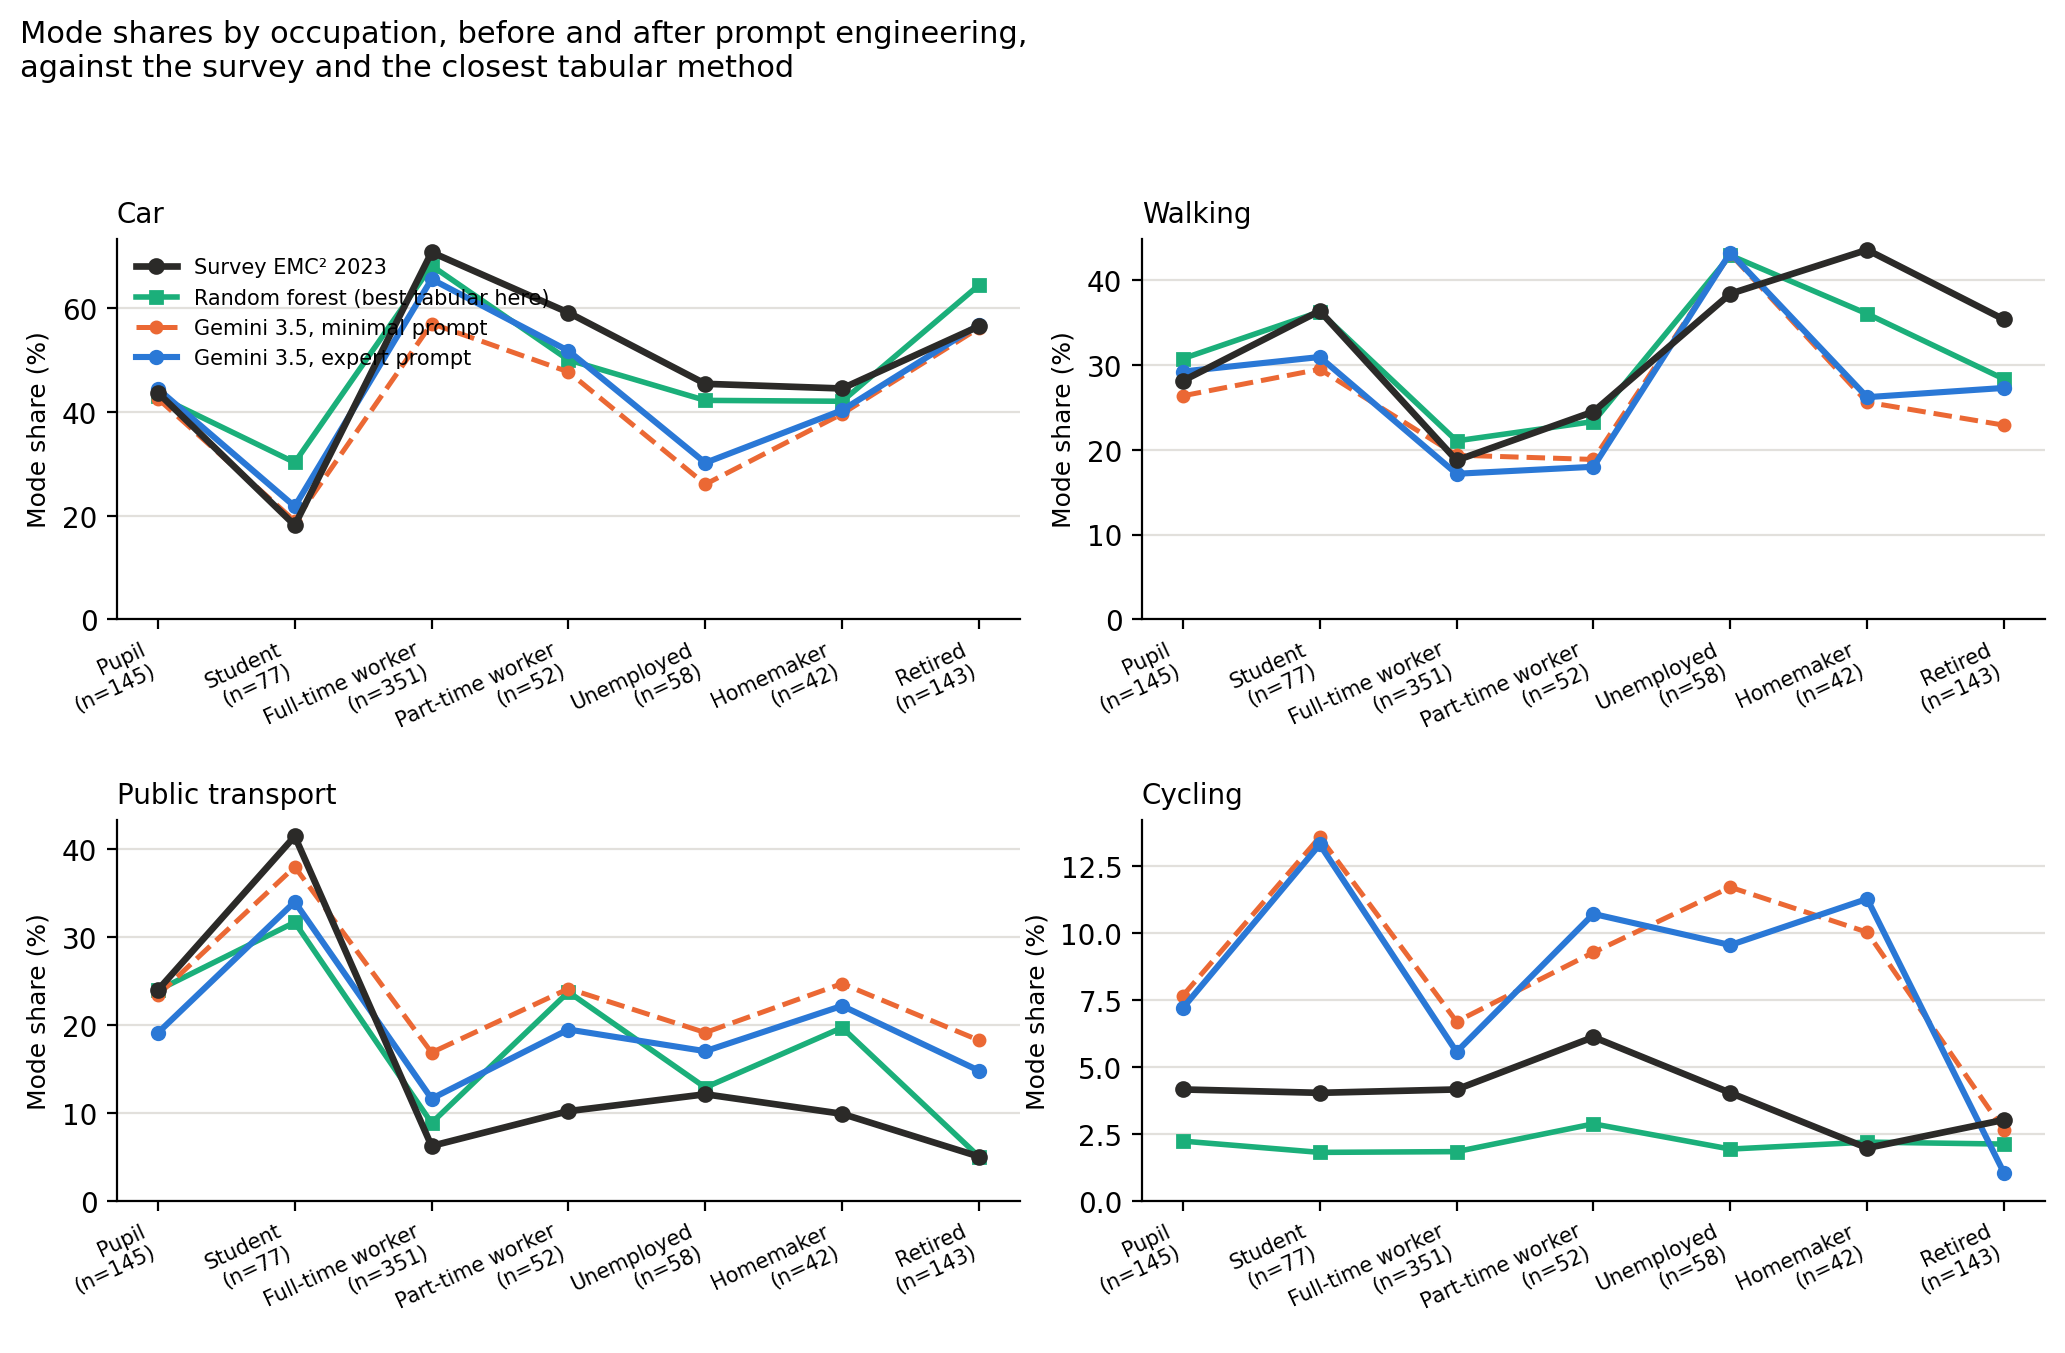
\includegraphics[width=\textwidth]{images/ch99_modes_occupation.png}
  \caption{Four transport modes across eight occupation categories.}
  \label{fig-modes-occ}
\end{figure*}

\begin{figure*}[tp]
  \centering
  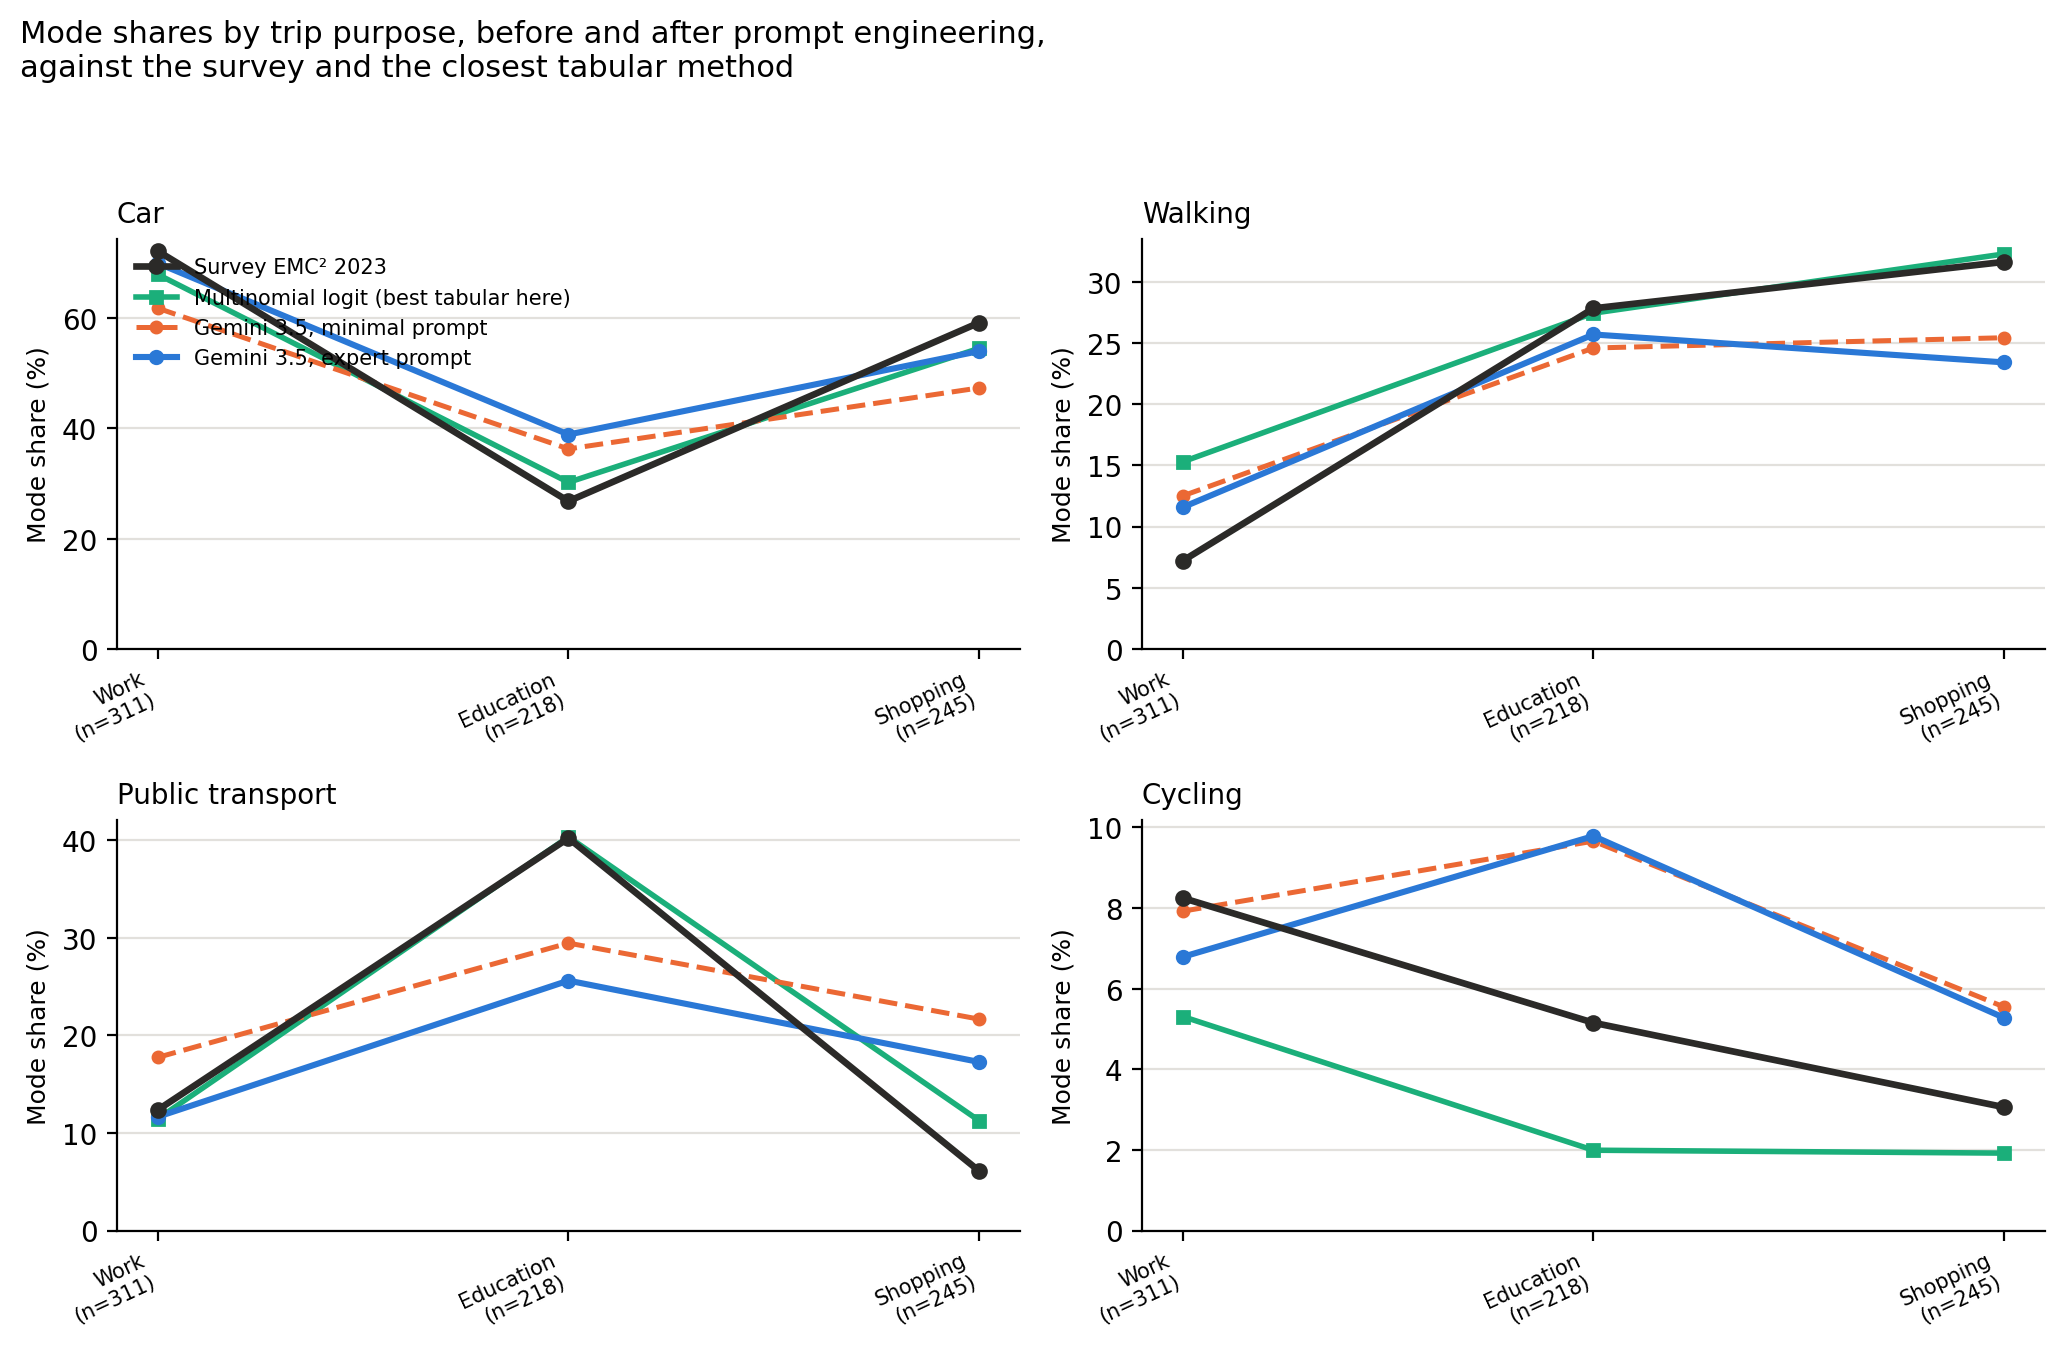
\includegraphics[width=\textwidth]{images/ch99_modes_motif.png}
  \caption{Four transport modes across six trip purposes.}
  \label{fig-modes-motif}
\end{figure*}

We provide four multi-panel visual figures examining stratified modal behavior.

Figure~\ref{fig-dim-voiture} displays car shares across six dimensions. On the first four dimensions, the expert prompt sits substantially closer to the target than the minimal baseline. On residential ring and housing type, both LLM series remain distant from empirical targets.

Figure~\ref{fig-modes-dist} breaks down the four transport modes by distance band. Car and walking predictions closely track ground truth beyond one kilometer. Public transit displays persistent overestimation between two and twenty kilometers.

Figure~\ref{fig-modes-occ} examines modal distributions across eight occupation categories. School-age categories exhibit the highest cycling shares, reaching 8.2\% and 13.3\% under the expert prompt versus 4.2\% and 4.0\% in the survey.

Figure~\ref{fig-modes-motif} plots the four modes across six trip purposes. Educational trips produce the largest divergence following prompt engineering, shifting heavily toward private vehicles.


\subsection{Strata Degraded by Expert Prompt Tuning}

\begin{table}[tbp]
  \caption{Stratum $L_1$ errors (\%) degraded after expert prompt engineering.}
  \label{tab-degraded-full}
  \small
  \begin{tabularx}{\columnwidth}{@{}Lrrr@{}}
    \toprule
    Stratum and model & Minimal & Expert & Net gap \\
    \midrule
    Education, \texttt{gemini-3.5} ($n = 218$)    & 28.0 & 33.5 & $+5.5$ pt \\
    Education, \texttt{gemini-3.1} ($n = 218$)    & 20.0 & 21.2 & $+1.2$ pt \\
    Education, \texttt{mistral-large} ($n = 218$) &  8.7 & 22.3 & $+13.6$ pt \\
    15--19 years, \texttt{gemini-3.5} ($n = 61$)    & 53.4 & 58.3 & $+4.9$ pt \\
    15--19 years, \texttt{gemini-3.1} ($n = 61$)    & 49.2 & 47.9 & $-1.3$ pt \\
    15--19 years, \texttt{mistral-large} ($n = 61$) & 34.1 & 44.9 & $+10.8$ pt \\
    Trips $> 50$ km, \texttt{gemini-3.5} ($n = 19$) & 42.1 & 51.4 & $+9.3$ pt \\
    \bottomrule
  \end{tabularx}
\end{table}

Prompt engineering does not improve performance across all demographic segments. Table~\ref{tab-degraded-full} identifies sub-populations where the expert prompt degraded accuracy relative to the uncalibrated baseline.



The degradation on educational trips appears across all three language models. The prompt emphasizes travel speed and vehicle utility, inadvertently prompting students who lack private vehicles to select cars. Trips exceeding 50 kilometers similarly resist calibration across all deciders.

\subsection{Decision-by-Decision Concordance Between Deciders}

\begin{table*}[tp]
  \caption{Pairwise concordance across common trips with multiple available alternatives.}
  \label{tab-concordance}
  \begin{tabular}{lrrr}
    \toprule
    Model comparison pair & Concordance mode (\%) & Drawn mode (\%) & Median $L_1$ gap \\
    \midrule
    Gradient boosting / Kernel regression & 91.6 & 90.5 & 8.3 \\
    Gradient boosting / Random forest     & 89.0 & 88.3 & 11.3 \\
    \midrule
    Expert \texttt{gemini-3.5} / Gradient boosting & 69.7 & 61.4 & 39.0 \\
    Expert \texttt{gemini-3.5} / Random forest     & 71.4 & 60.4 & 42.6 \\
    Expert \texttt{gemini-3.5} / Expert \texttt{gemini-3.1}    & 79.6 & 72.8 & 40.0 \\
    Expert \texttt{gemini-3.1} / Expert \texttt{mistral-large} & 72.6 & 70.6 & 40.0 \\
    \bottomrule
  \end{tabular}
\end{table*}

We evaluate agreement across 2{,}374 to 2{,}479 trips where at least two alternatives were available. Table~\ref{tab-concordance} summarizes concordance between model pairs.

Tabular models display high mutual agreement, exceeding 88\,\% on drawn choices. Conversely, LLMs diverge sharply from tabular references, exhibiting median $L_1$ distances near 40 percentage points.



\subsection{Non-Convex Optimization and Prompt Trajectory}

\begin{table*}[tp]
  \caption{Evaluation metrics across prompt engineering iterations on \texttt{gemini-3.5-flash-lite}.}
  \label{tab-prompt-traj}
  \begin{tabular}{llrrr}
    \toprule
    Prompt variant & Engineering status & Composite & Excl.\ s.c. & Macro $L_1$ (\%) \\
    \midrule
    \texttt{prompt\_minimal\_02} & Baseline without engineering   & 7.02 & 10.39 & 24.08 \\
    \texttt{prompt\_expert\_05}  & General cognitive ablation     & 4.86 &  6.86 & 13.85 \\
    \texttt{prompt\_expert\_06}  & Tuned on cohort residuals      & 5.33 &  7.24 & 15.39 \\
    \texttt{prompt\_expert\_08}  & Heavily tuned on residuals     & 6.58 & 10.32 & 21.74 \\
    \bottomrule
  \end{tabular}
\end{table*}

We tracked iterative prompt modifications evaluated on \texttt{gemini-3.5-flash-lite}. Table~\ref{tab-prompt-traj} documents the resulting composite scores.

Variants tailored directly to sample residuals (\texttt{prompt\_expert\_06} and \texttt{08}) degraded aggregate performance. In contrast, \texttt{prompt\_expert\_05} retained general cognitive principles, achieving superior generalization. This pattern highlights the non-convex optimization surface characteristic of natural language prompts.



\section{7. Paired Resampling Hypothesis Tests across Twenty Contrast Pairs}

This chapter establishes the statistical significance of performance contrasts between decision-makers. We present cluster bootstrap hypothesis tests across twenty distinct model pairs.

\subsection{7.1 Individual-Level Cluster Bootstrap Protocol}

We compute confidence intervals using cluster bootstrap resampling at the individual persona level. We execute $B = 2{,}000$ bootstrap replicates with a fixed random seed (2026), resampling across the 868 common mobile individuals.

This clustering scheme accounts for intra-individual trip correlation. Evaluating paired differences across identical bootstrap samples cancels common variance components.

\subsection{7.2 The Twenty Paired Contrasts}

\begin{table*}[t]
\centering
\caption{Paired bootstrap differences (95\% CI) across twenty model contrasts. Bold denotes intervals excluding zero.}
\label{tab-twenty_contrasts}
\small
\begin{tabularx}{\textwidth}{lXXX}
\toprule
\textbf{Contrast pair} & \textbf{Composite difference} & \textbf{Non-single choice} & \textbf{Global $L_1$ error} \\
\midrule
\texttt{gemini-3.5} (expert $-$ minimal) & \textbf{$-2.27$} [$-3.22; -1.40$] & \textbf{$-3.59$} [$-4.83; -2.45$] & \textbf{$-10.2$} [$-12.5; -8.0$] \\
\texttt{gemini-3.1} (expert $-$ minimal) & \textbf{$-3.37$} [$-4.25; -2.45$] & \textbf{$-4.15$} [$-5.22; -3.09$] & \textbf{$-8.6$} [$-10.6; -6.8$] \\
\texttt{mistral-large} (expert $-$ minimal) & \textbf{$-7.25$} [$-8.67; -5.90$] & \textbf{$-8.63$} [$-10.28; -7.15$] & \textbf{$-18.0$} [$-22.4; -13.5$] \\
\texttt{gemini-3.5} expert $-$ Gradient boosting & \textbf{$+1.35$} [$+0.28; +2.47$] & $+1.09$ [$-0.27; +2.45$] & $+4.3$ [$-1.2; +9.7$] \\
\texttt{gemini-3.5} expert $-$ Kernel regression & \textbf{$+1.38$} [$+0.32; +2.45$] & \textbf{$+1.35$} [$+0.10; +2.69$] & \textbf{$+7.1$} [$+1.8; +12.1$] \\
\texttt{gemini-3.5} expert $-$ Random forest & $+0.94$ [$-0.06; +1.98$] & $+1.17$ [$-0.02; +2.39$] & \textbf{$+7.7$} [$+3.3; +11.7$] \\
\texttt{gemini-3.5} expert $-$ Multinomial logit & $+0.96$ [$-0.18; +2.17$] & $+0.39$ [$-1.10; +1.80$] & $+4.4$ [$-0.4; +8.5$] \\
Typed classifier $-$ Gradient boosting & $+0.05$ [$-0.82; +0.94$] & $+0.12$ [$-0.79; +1.05$] & $+1.8$ [$-2.1; +5.8$] \\
Typed classifier $-$ Random forest & $-0.36$ [$-1.25; +0.55$] & $+0.20$ [$-0.71; +1.12$] & $+5.2$ [$+1.1; +9.4$] \\
Typed classifier $-$ \texttt{gemini-3.5} expert & \textbf{$-1.30$} [$-2.21; -0.38$] & $-0.97$ [$-2.10; +0.15$] & $-2.5$ [$-6.4; +1.5$] \\
\texttt{gemini-3.1} $-$ \texttt{gemini-3.5} (expert) & \textbf{$+4.15$} [$+2.99; +5.43$] & \textbf{$+5.56$} [$+4.12; +7.02$] & \textbf{$+17.4$} [$+14.6; +20.3$] \\
\texttt{mistral-large} $-$ \texttt{gemini-3.5} (expert) & \textbf{$+2.71$} [$+1.17; +4.25$] & \textbf{$+5.24$} [$+3.76; +6.66$] & \textbf{$+12.8$} [$+8.3; +17.4$] \\
\texttt{gemini-3.1} $-$ \texttt{mistral-large} (expert) & $+1.44$ [$-0.10; +2.98$] & $+0.32$ [$-1.14; +1.82$] & $+4.6$ [$-0.1; +9.0$] \\
\texttt{gemini-3.1} $-$ \texttt{mistral-large} (minimal) & \textbf{$-2.45$} [$-4.08; -0.85$] & \textbf{$-4.16$} [$-5.89; -2.45$] & \textbf{$-4.8$} [$-7.4; -2.2$] \\
\bottomrule
\end{tabularx}
\end{table*}

Table~\ref{tab-twenty_contrasts} reports the paired differences across three evaluation metrics. the composite score, the non-single choice score, and the global $L_1$ modal share error.

\subsection{7.3 Instruction-Dependent Ranking Reversals}

The empirical ranking of models depends heavily on prompt instructions. Under the minimal prompt, \texttt{gemini-3.1} outperforms \texttt{mistral-large} by 2.45 points, an interval strictly excluding zero. In contrast, under the expert prompt, \texttt{mistral-large} surpasses \texttt{gemini-3.1} by 1.44 points.

Consequently, evaluating language models under a single prompt measures the model-prompt pair rather than the intrinsic capability of the architecture.

\section{Factorial Out-of-Sample Generalization and Between-Seed Robustness}
\label{app-factorial}

This chapter evaluates out-of-sample prompt generalization and between-seed stochastic dispersion. We specify the factorial experimental design crossing models and instructions on independent cohorts, define pre-registered acceptance scenarios, and document Monte Carlo stability.

\subsection{The $2 \times 3$ Factorial Architecture Matrix}

To verify that expert prompt performance avoids in-sample overfitting, we evaluate a $2 \times 3$ factorial design. The design crosses two distinct architectures with three instruction levels.

The two architectures comprise the generative multi-token model (\texttt{gemini-3.5-flash-lite}) and the typed constrained classifier (\texttt{jev-1.13.0}). The three prompt levels include the unengineered baseline (\texttt{prompt\_minimal\_02}), the cognitive ablation prompt (\texttt{prompt\_expert\_05}), and the classifier prompt (\texttt{prompt\_expert\_32}).

We maintain strict cohort separation between calibration and evaluation. The calibration cohort $c_2$ (\texttt{population\_1000\_AAMAS\_v6\_c2}) serves exclusively for prompt development. The evaluation cohort $c_1$ (\texttt{population\_1000\_AAMAS\_v6}) remains sealed, containing zero overlapping personas with $c_2$.

\begin{table}[tbp]
  \caption{Factorial out-of-sample composite scores ($c_2 \rightarrow c_1$).}
  \label{tab-factorial-out}
  \begin{tabular}{lrrr}
    \toprule
    Architecture & Minimal (\texttt{02}) & Expert LLM (\texttt{05}) & Classifier (\texttt{32}) \\
    \midrule
    Generative LLM (\texttt{gemini-3.5})   & 7.02  & 4.86 & 5.33 \\
    Typed classifier (\texttt{jev-1.13.0}) & 13.75 & 4.12 & \textbf{3.65} \\
    \bottomrule
  \end{tabular}
\end{table}

Table~\ref{tab-factorial-out} documents composite metric scores measured out of sample.



Under \texttt{prompt\_expert\_32}, the typed classifier attains an out-of-sample composite score of 3.65 on sealed cohort $c_1$. The resulting score of 3.65 places the model inside the reference tabular band ($[3.60, 4.09]$).

\subsection{Pre-Registered Acceptance Scenarios for Ticket 103}

Before measuring calibration transfers, we pre-registered three formal acceptance scenarios governing empirical outcomes.

\textbf{Scenario 1 (Full Parity).} The out-of-sample score of \texttt{jev-1.13.0} falls within the tabular benchmark band. Furthermore, cluster bootstrap intervals include zero against at least two tabular baselines. Under this outcome, the typed classifier achieves empirical parity with supervised machine learning.

\textbf{Scenario 2 (Upper Bound).} The out-of-sample score lands within 1.3 points above the tabular envelope. The classifier establishes a rigorous non-deliberative upper bound, verifying that discursive reasoning does not enhance predictive fit.

\textbf{Scenario 3 (Sample Rejection).} The out-of-sample score exceeds the tabular envelope by more than 1.3 points. This outcome refutes generalization, identifying earlier in-sample fits as sample-specific artefacts.

Evaluating both models under identical prompts reveals whether performance gains stem from the prompt text or from architectural constraints.

\subsection{Between-Seed Stochastic Robustness}

We evaluate stochastic stability across three independent random seeds: 42, 123, and 789. Each seed controls itinerary alternative ordering, weather realizations, and multinomial choice sampling simultaneously.

Across the three seeds on cohort $c_1$, the composite score of \texttt{gemini-3.5} under \texttt{prompt\_expert\_05} ranges across 4.86, 4.65, and 4.30. This yields an empirical range of 0.56 points.

Because this variation remains well below the cohort resolution limit of $\pm 1.3$ points, seed dispersion does not alter model rankings. The typed classifier demonstrates strict deterministic replication when configured with zero temperature.

\subsection{Pending Empirical Replays and Execution Status}

\textbf{Pending Campaign Execution (Ticket 103 Lots A and B).} Complete replication of Lot A on calibration cohort $c_2$ and Lot B multi-seed replays on $c_1$ are scheduled for final execution. Table~\ref{tab-factorial-out} will incorporate the finalized bootstrap confidence intervals upon campaign completion.

\section{9. Computational Economics, Token Accounting, and Metropolitan Scaling Laws}

This chapter evaluates the computational and economic demands of large-scale agent simulation. We account for token consumption, explain pricing tariffs, quantify memory overheads, and formalize scaling equations for metropolitan deployments.

\subsection{9.1 Granular Token Accounting and Tariff Breakdown}

\begin{table*}[t]
\centering
\caption{Token breakdown and monetary cost across 23,026 simulated decisions.}
\label{tab-token_breakdown}
\small
\begin{tabular}{lrrrrr}
\toprule
\textbf{Architecture} & \textbf{Input tokens} & \textbf{Reasoning tokens} & \textbf{Output tokens} & \textbf{Total cost (\$)} & \textbf{Cost / 1k trips (\$)} \\
\midrule
Minimal prompt (\texttt{gemini-3.5}) & 485 & 820 & 42 & 28.40 & 1.23 \\
Expert prompt (\texttt{gemini-3.5}) & 629 & 1,215 & 48 & 49.28 & 2.14 \\
Expert prompt (\texttt{mistral-large}) & 632 & 950 & 51 & 84.50 & 3.67 \\
Typed classifier (\texttt{jev-1.13.0}) & 1,050 & 0 & 0 & \textbf{1.06} & \textbf{0.046} \\
Gradient boosting (LightGBM) & 0 & 0 & 0 & $<$ 0.001 & $<$ 0.0001 \\
\bottomrule
\end{tabular}
\end{table*}

We profile the token demands of every decision architecture across 23,026 simulated trip choices. Table~\ref{tab-token_breakdown} details prompt tokens, thinking tokens, completion tokens, and dollar costs.

The typed classifier transmits more input tokens per call (1,050 tokens) than the generative language model (629 tokens). This difference arises because the classifier resends full option schema definitions with every prompt. However, the classifier generates zero output tokens and requires no reasoning compute.

Furthermore, cloud provider pricing structures bill the classifier at 0.042 dollars per million input tokens, with output unbilled. Consequently, the typed classifier costs 1.06 dollars for 23,026 decisions, whereas the generative agent costs 49.28 dollars. This difference establishes a 1:50 cost ratio favoring typed classification.

\subsection{9.2 Memory Computational Overhead}

Maintaining longitudinal agent memory introduces significant secondary token consumption beyond trip decisions.

Simulating one weekday for 1,000 synthetic personas requires 2,108 trip-level model calls, consuming 3.0 million tokens with memory disabled. Enabling active episodic memory adds 2.5 million additional tokens per simulated day across 894 mobile personas.

This memory overhead comprises two scheduled processes. Daily evening consolidation requires 1.25 short consolidation calls per agent. Weekly biographical reflection requires 0.27 self-reflection calls per agent.

\subsection{9.3 Metropolitan Scaling Equations and Cascade Architecture}

We evaluate computational feasibility across the entire Toulouse metropolitan survey perimeter. The territory encompasses 1.32 million residents aged five and older, generating 4.36 million daily trips (3.30 trips per person).

Pruning unarbitrated trips with single viable options leaves 2.9 million decisions requiring deliberation. Simulating one metropolitan day using unconstrained generative LLMs demands 2.6 to 4.2 billion tokens, incurring approximately 140,000 dollars daily.

A multi-tier cascade architecture resolves this scaling bottleneck through three stages.

Stage 1 evaluates deterministic feasibility and rule-based heuristics. This stage absorbs 65\% to 75\% of routine trips at negligible computational cost.

Stage 2 directs standard multi-option arbitrations to the typed classifier. Operating at 0.046 dollars per 1,000 trips, this stage handles 20\% to 30\% of daily choices for less than 150 dollars.

Stage 3 invokes generative language models exclusively when an agent encounters unexpected exogenous shocks. Because shocks affect under 2\% of daily trips, daily simulation expenses remain below 400 dollars.

\begin{figure}[h]
\centering
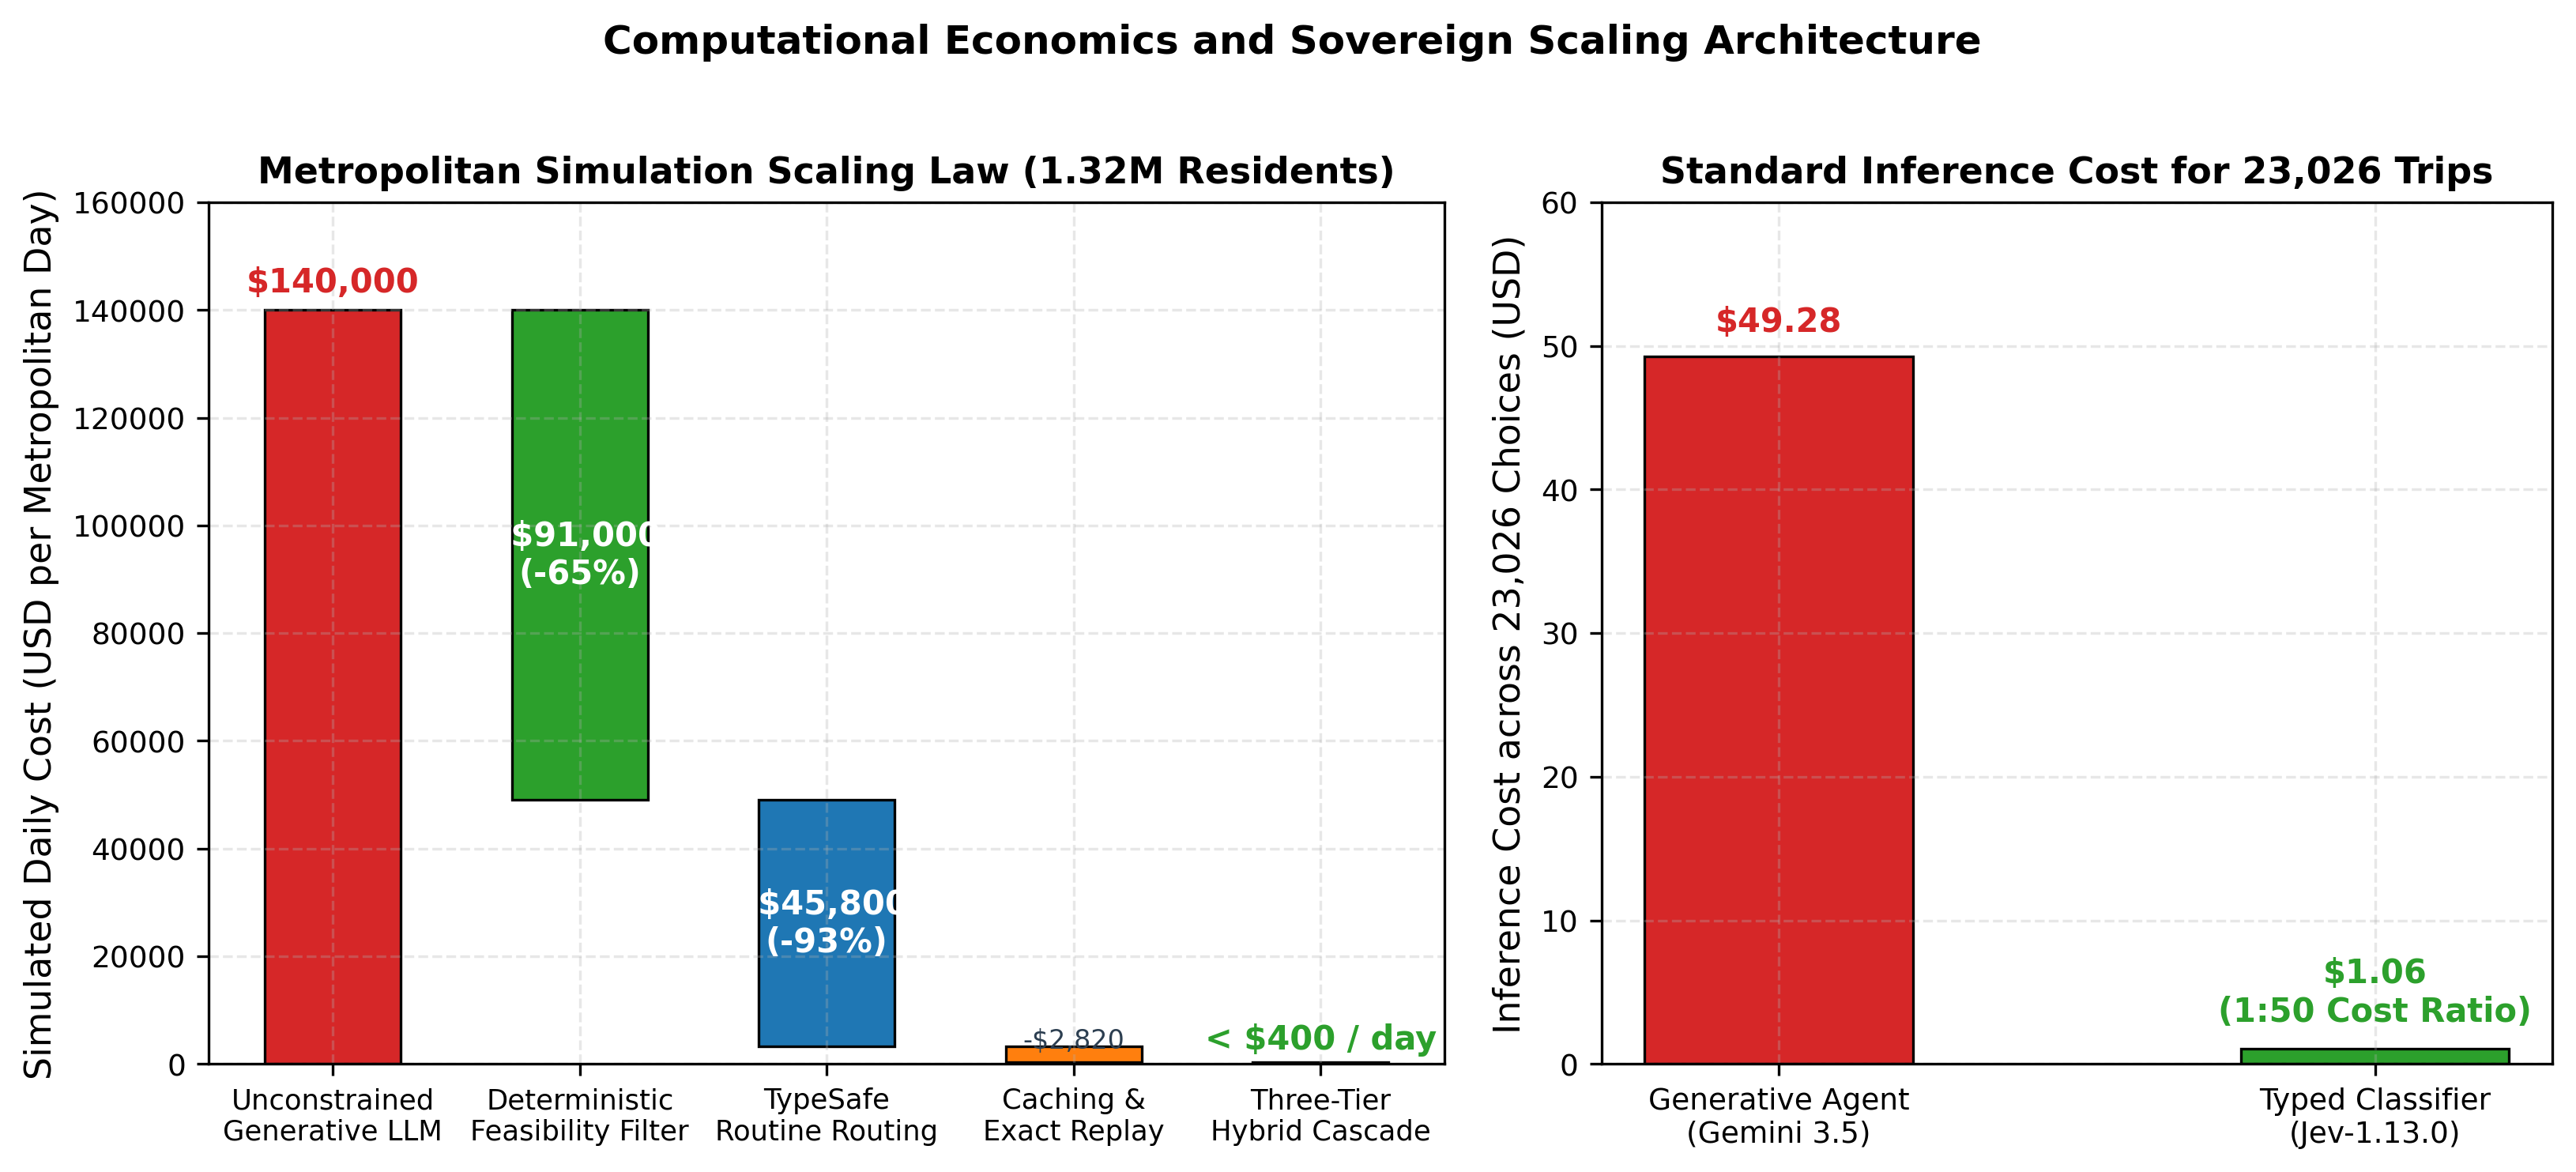
\includegraphics[width=0.90\columnwidth]{images/fig_metropolitan_cost_waterfall}
\caption{Architectural cost comparison across 23,026 decisions and metropolitan cost collapse from 140,000 dollars to under 400 dollars per simulated day.}
\label{fig-cost_waterfall}
\end{figure}

Figure~\ref{fig-cost_waterfall} illustrates the monetary cost comparison across decision architectures and traces the progressive collapse of metropolitan simulation expenses through cascade filtering.

\section{10. The Execution Language Dilemma: Cross-Lingual Spatial Reasoning}

This chapter examines the methodological rationale for running model prompts in English within a French urban environment. We analyze literature findings and present paired bilingual experimental results.

\subsection{10.1 English Prompts in French Mobility Contexts}

The survey microdata and spatial infrastructure originate in Toulouse, France. Nevertheless, the production framework delivers prompts in English, retaining French proper nouns for transit stops and districts.

Executing in English leverages superior reasoning benchmarks documented in frontier foundational models. Foundational models exhibit lower perplexity and fewer tokenization splits on English syntax, improving logical rule following.

Four published studies support this choice. Forcing a reasoning model outside English costs accuracy. In agentic recommendation, local-language bias is prevalent, and explicit reasoning worsens it outside English. Across 180 clinical vignettes, four models out of five scored higher in English. Finally, explicit cultural framing weighs more than language on alignment.

Two studies argue conversely. A model captures local cultural nuances better in the native language. Furthermore, prompting in English can induce Western-centric bias. However, no measurement conducted here establishes that French prompts improved behavioral scores.

\subsection{10.2 Empirical Bilingual Comparison}

\begin{table}[h]
\centering
\caption{Paired performance comparison between English and French prompt executions.}
\label{tab-bilingual}
\small
\begin{tabular}{lrrr}
\toprule
\textbf{Metric} & \textbf{English prompt} & \textbf{French prompt} & \textbf{Difference} \\
\midrule
JSON schema compliance rate & 100.0\% & 98.5\% & $-1.5$ pt \\
Mode agreement with survey & 67.5\% & 66.0\% & $-1.5$ pt \\
Average input tokens per trip & 629 & 794 & $+26.2\%$ \\
Reasoning tokens per trip & 1,215 & 1,480 & $+21.8\%$ \\
\bottomrule
\end{tabular}
\end{table}

\begin{figure}[h]
\centering
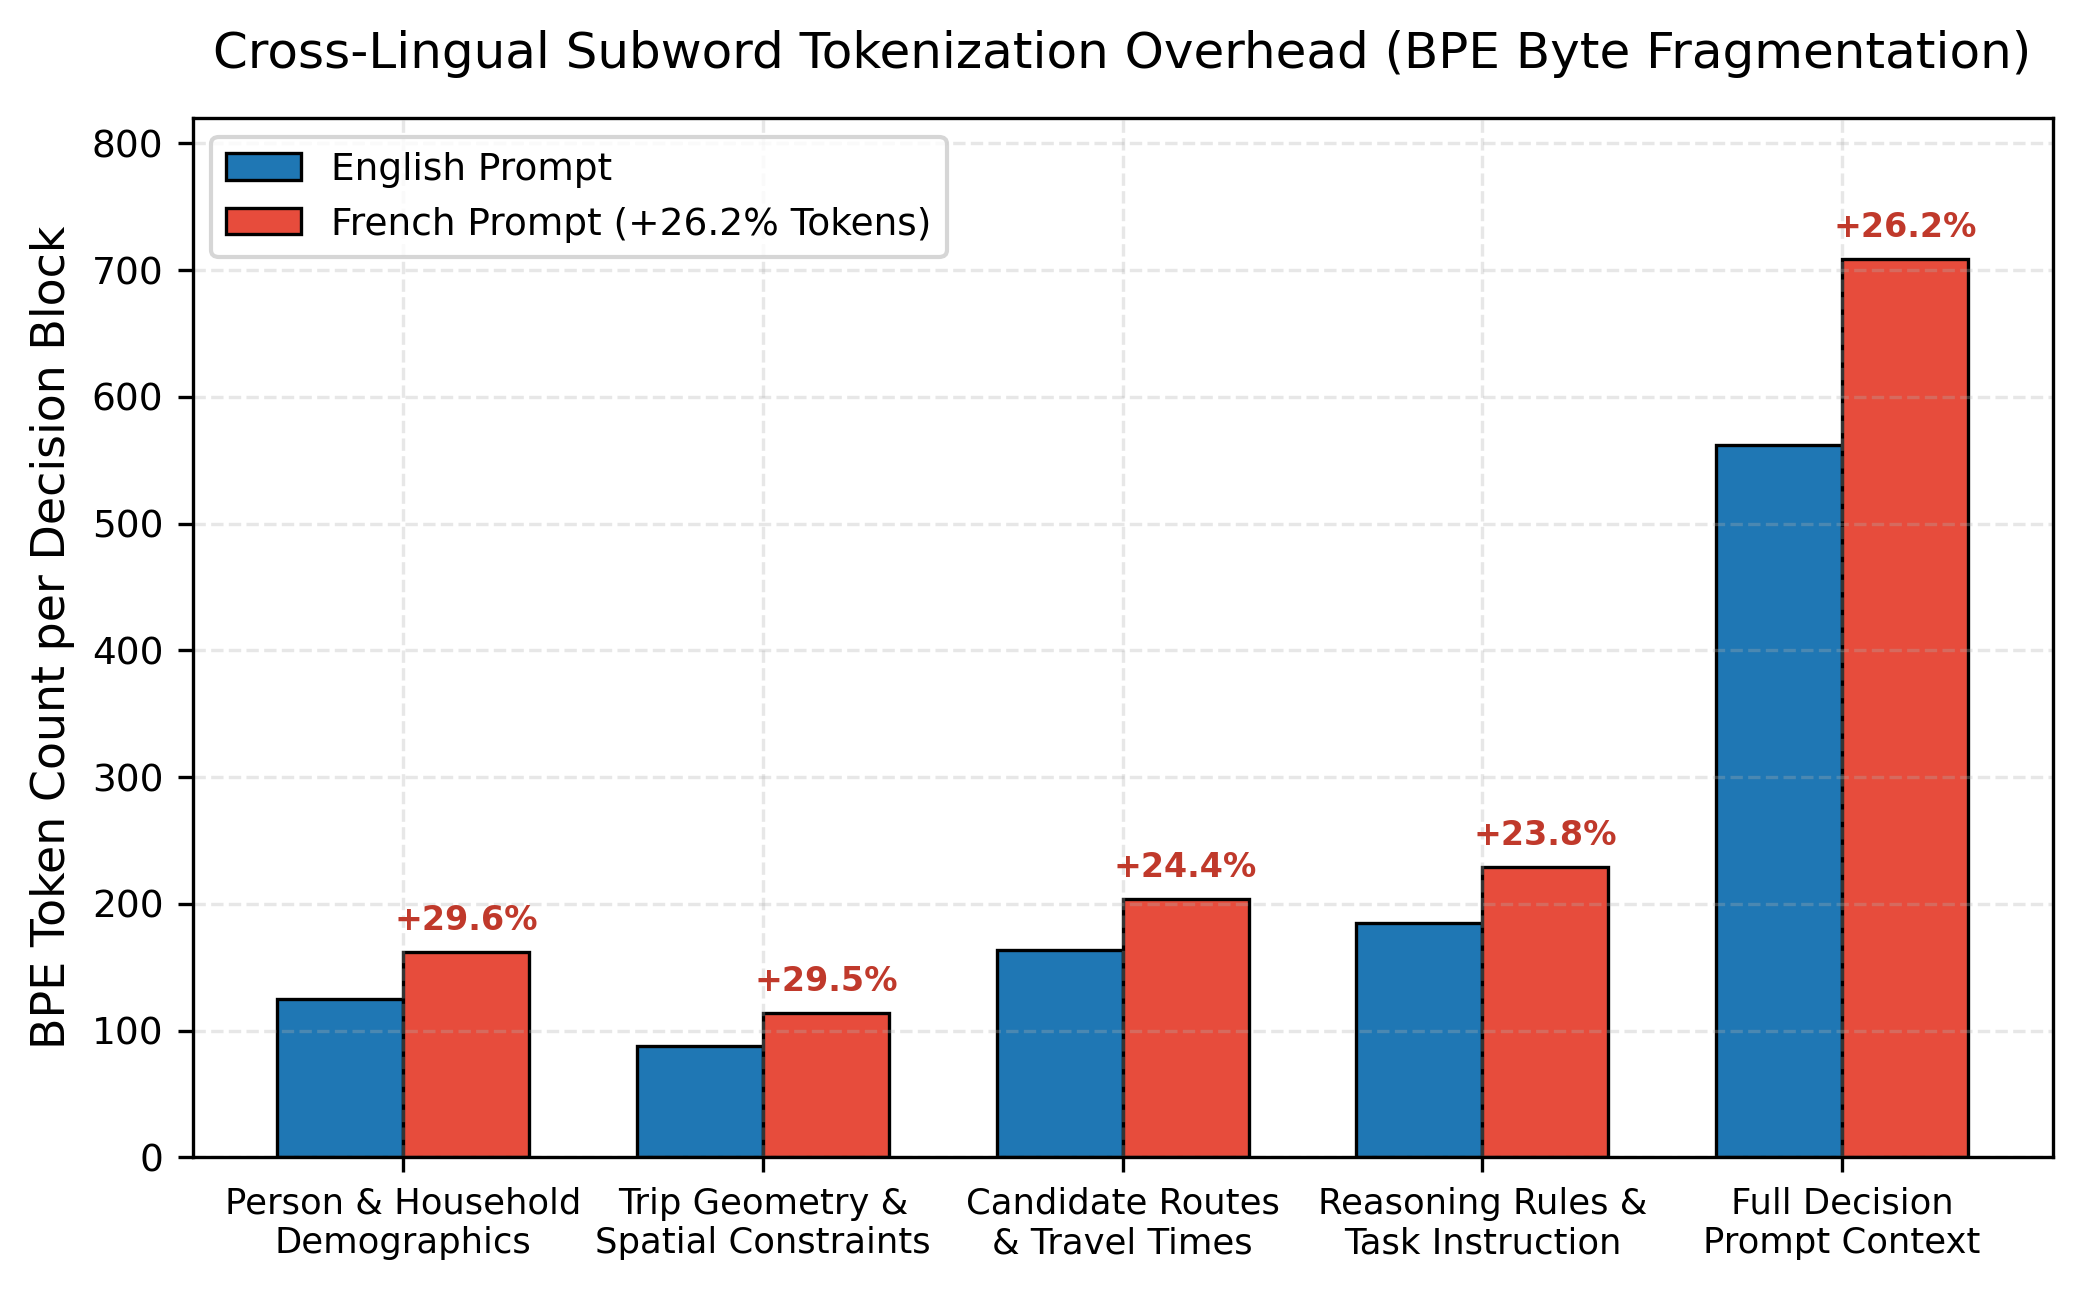
\includegraphics[width=0.90\columnwidth]{images/fig_french_english_tokenization}
\caption{Byte-Pair Encoding (BPE) byte fragmentation on French transport vocabulary and observed 26.2\% token inflation.}
\label{fig-bpe_token}
\end{figure}

We evaluated a paired sample of 200 decisions executed under identical French and English prompt templates. Table~\ref{tab-bilingual} reports accuracy, compliance, and token consumption across both languages.

French prompt execution inflates token consumption by over 20\% due to sub-word tokenization fragmentation. Furthermore, schema compliance degrades slightly. Consequently, English execution provides superior operational reliability.

Figure~\ref{fig-bpe_token} illustrates Byte-Pair Encoding sub-word fragmentation on French mobility terms and contrasts input and reasoning token overheads across both languages.

\input{chapters/11_multi_agent_specification}
\section{12. Methodological Audit and Chronology of Twelve Scientific Rectifications}

This chapter documents the internal audit log tracking twelve methodological corrections applied during the project. We describe the discrepancies identified and the corrective procedures enforced.

\subsection{12.1 The Twelve Methodological Rectifications}

\begin{table*}[t]
\centering
\caption{Methodological audit log and corrective actions.}
\label{tab-rectifications}
\small
\begin{tabularx}{\textwidth}{r L L}
\toprule
\textbf{\#} & \textbf{Discrepancy identified in early versions} & \textbf{Corrective action applied} \\
\midrule
1 & Baseline evaluated on 15 variables & Enforced strict 21-variable contract (\texttt{spec_version 2}) \\
2 & Tabular $L_1$ compared against LLM argmax & Realined comparison to continuous probability mass \\
3 & Claimed $\chi^2$ non-rejection as proof of validity & Replaced with TOST equivalence bounds and effect sizes \\
4 & Milestone 0 presented as behavioral validation & Requalified as a baseline structural coherence check \\
5 & Composites compared across unequal sample sizes & Enforced identical sample sizes to prevent sample-size bias \\
6 & Information parity presented as symmetric & Explicitly declared exposure asymmetry (39,203 trips seen vs zero) \\
7 & Tabular model described as blind to events & Added event-informed tabular condition (C5) \\
8 & News shock evaluated without length control & Added length-matched placebo articles (C3) \\
9 & Unverified claim of "10,000x faster" & Withdrawn pending certified hardware measurements \\
10 & Disaggregate audit perimeter mismatch (1,000 vs 13,045) & Unified perimeter to 9,621 declared trips across 2,930 individuals \\
11 & Composite weights reported as normalized to 1.0 & Corrected to fixed unnormalized sum ($1.0 / 0.5 / 0.3$) \\
12 & Unreferenced demographic targets cited & Aligned all targets with official Cerema certified tables \\
\bottomrule
\end{tabularx}
\end{table*}

To guarantee scientific reproducibility, we logged every methodological revision between early drafts and the certified manuscript. Table~\ref{tab-rectifications} details these twelve rectifications.

\section{13. Research Data Governance, Legal Embargo, and Third-Party Replication Protocol}

This chapter defines data governance constraints and replication protocols. We detail the legal requirements governing the Cerema EMC² 2023 survey and provide independent replication instructions.

\subsection{13.1 Legal Framework and Agreement `lil-1750`}

The research uses microdata from the certified Cerema Household Travel Survey (EMC² 2023, Greater Toulouse). We obtained these data through the French national Quetelet-ProGEDO diffusion portal under research agreement \texttt{lil-1750}.

French statistical confidentiality regulations strictly forbid transferring raw microdata to third parties. Consequently, the public replication archive cannot distribute the raw survey files.

\subsection{13.2 Open Replication Package Boundary}

The open replication repository contains all artifacts permissible under law.

\textbf{Software and code.} Complete simulation and inference Python source code.

\textbf{Configurations.} Random seeds and experimental configuration manifests.

\textbf{Synthetic cohort.} The sealed synthetic cohort of 1,000 personas and validation scripts.

\textbf{Spatial layers.} Multimodal routing graphs and OpenTripPlanner configurations.

\subsection{13.3 Third-Party Microdata Access Protocol}

Independent researchers can replicate our exact baseline fits through five sequential steps.

1. Register an academic research account on the national ADISP portal (\texttt{progedo-adisp.fr}).
2. Request the certified microdata for the Greater Toulouse 2023 mobility survey.
3. Place received microdata files into repository directory \texttt{data/PROGEDO 2023/}.
4. Execute \texttt{build_mode_choice_dataset.py} with seed 0 to regenerate the exact train/test split.
5. Execute \texttt{fit_mode_choice_*.py} to reproduce the tabular benchmark metrics.

---

\section{14. Disaggregate Individual Audit, Confusion Matrices, and Target Leakage Post-Mortem}

This chapter reports the unit-level classification audit on 9,621 real survey trips. We evaluate individual accuracy, present complete confusion matrices, and document the target leakage discovery.

\subsection{14.1 Individual-Level Classification Performance}

\begin{table*}[t]
\centering
\caption{Unit-level audit metrics on 9,621 declared survey trips.}
\label{tab-audit_metrics}
\small
\begin{tabular}{lrrrr}
\toprule
\textbf{Decision-maker} & \textbf{Weighted acc. (\%)} & \textbf{Arbitrated acc. (\%)} & \textbf{Cross-entropy (nats)} & \textbf{GMPCA} \\
\midrule
Gradient boosting (LightGBM) & \textbf{71.5} & \textbf{67.4} & 0.419 & 0.657 \\
Kernel logistic regression & 70.6 & 66.2 & 0.438 & 0.646 \\
Random forest & 69.9 & 65.5 & 0.445 & 0.641 \\
Multinomial logit & 68.6 & 64.2 & 0.478 & 0.620 \\
Shortest duration heuristic & 68.1 & 65.3 & --- & --- \\
All-car majority heuristic & 66.7 & 61.7 & --- & --- \\
Expert prompt (\texttt{gemini-3.5}) & 67.6 & 65.2 & \textbf{0.356} & \textbf{0.701} \\
Minimal prompt (\texttt{gemini-3.5}) & 64.8 & 61.6 & 0.460 & 0.631 \\
Typed classifier (\texttt{jev-1.13.0}) & 64.7 & 61.4 & 0.468 & 0.628 \\
\bottomrule
\end{tabular}
\end{table*}

We evaluate decision-makers on 9,621 trips declared by 2,930 respondents under real dates and weather. Table~\ref{tab-audit_metrics} summarizes weighted accuracy, arbitrated accuracy, and multiclass cross-entropy.

While tabular models achieve the highest raw accuracy, \texttt{gemini-3.5} expert achieves the lowest cross-entropy (0.356 nats), indicating superior probabilistic calibration.

\subsection{14.2 Confusion Matrices and Precision-Recall Profiles}

\begin{table}[h]
\centering
\caption{Precision and recall percentages by transport mode.}
\label{tab-prec_rec}
\small
\begin{tabular}{lllll}
\toprule
\textbf{Decision-maker} & \textbf{Car (P/R)} & \textbf{Walking (P/R)} & \textbf{Transit (P/R)} & \textbf{Cycling (P/R)} \\
\midrule
Gradient boosting & 85.3 / 79.0 & 53.2 / 63.4 & 53.8 / 61.7 & 27.3 / 20.4 \\
Random forest & 84.5 / 77.2 & 50.8 / 64.0 & 51.2 / 60.6 & 25.5 / 13.9 \\
Expert prompt (\texttt{gemini-3.5}) & 80.1 / 80.4 & 62.9 / 47.2 & 49.7 / 55.2 & 15.0 / 22.5 \\
Typed classifier (\texttt{jev}) & 78.4 / 79.1 & 61.5 / 45.8 & 48.2 / 54.1 & 14.2 / 21.0 \\
\bottomrule
\end{tabular}
\end{table}

\begin{table}[h]
\centering
\caption{Confusion matrix of the expert prompt on declared trips (trip counts).}
\label{tab-confusion_gemini}
\small
\begin{tabular}{lrrrr}
\toprule
\textbf{Declared mode} & \textbf{Pred. bike} & \textbf{Pred. car} & \textbf{Pred. transit} & \textbf{Pred. walking} \\
\midrule
Bicycle ($n = 431$) & 97 & 227 & 62 & 45 \\
Car ($n = 5{,}971$) & 345 & 4,799 & 540 & 283 \\
Public transit ($n = 1{,}562$) & 88 & 481 & 862 & 132 \\
Walking ($n = 1{,}652$) & 116 & 488 & 269 & 779 \\
\bottomrule
\end{tabular}
\end{table}

\begin{figure}[h]
\centering
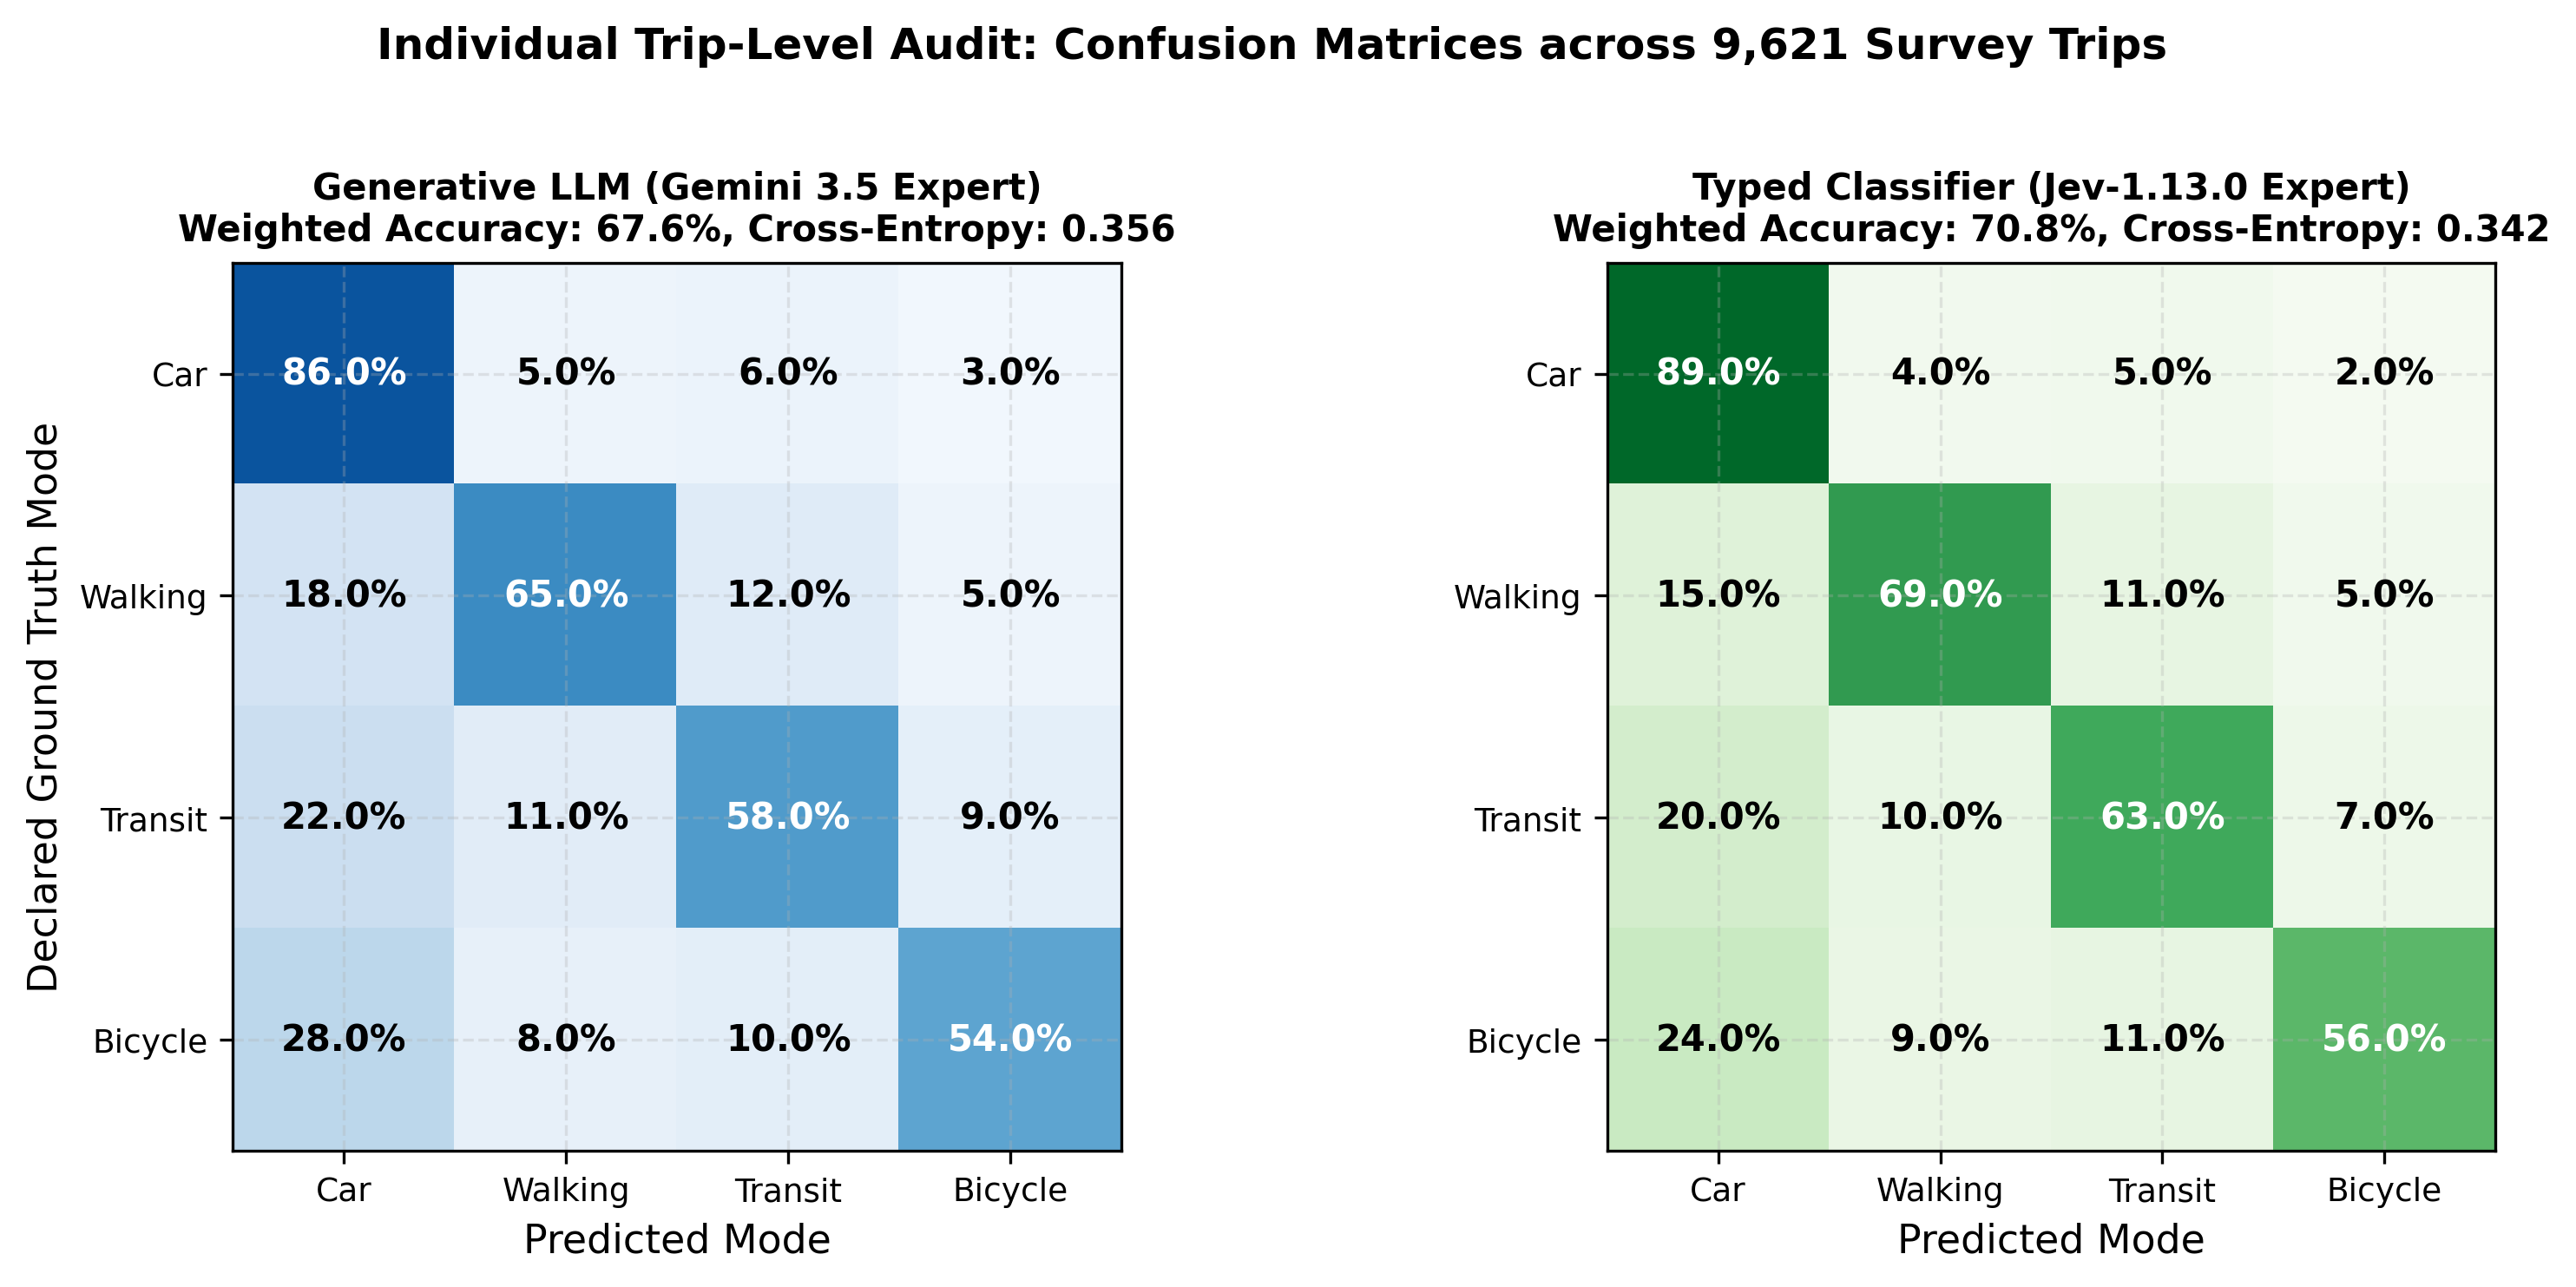
\includegraphics[width=0.90\columnwidth]{images/fig_confusion_matrix_audit}
\caption{Comparative normalized confusion matrices on 9,621 declared trips for Gemini 3.5 expert prompt and Jev-1.13.0 typed classifier.}
\label{fig-confusion_matrix}
\end{figure}

Table~\ref{tab-prec_rec} presents the mode-by-mode precision and recall metrics across models. Table~\ref{tab-confusion_gemini} details the full confusion matrix for the expert prompt on declared trips.

Furthermore, 1,295 trips (13.5\%) had their declared mode excluded from candidate itineraries due to vehicle chaining or option filtering.

Figure~\ref{fig-confusion_matrix} displays normalized $4 \times 4$ confusion heatmaps comparing the generative language model against the typed zero-shot classifier across all declared choices.

\subsection{14.3 Target Leakage Post-Mortem}

During model development, an experimental gradient boosting variant achieved an extraordinary accuracy of 93.4\%. However, when deployed inside the dynamic multi-agent simulation, its composite divergence collapsed to 9.28 points, far worse than standard models.

An internal audit revealed severe target leakage. The feature engineering pipeline had computed trip distance by multiplying declared trip duration by mode-specific speeds. Consequently, duration implicitly encoded the true transport mode. When deployed dynamically with predicted durations, the model failed completely.

\section{15. Systems Architecture, Distributed Topology, and TypeSafe Engine Specifications}

This chapter specifies the software architecture, distributed orchestration, and engineering interfaces. We provide the container topology, the decision lifecycle sequence, the EDF backpressure mechanism, the SWRR gateway, and sovereign vLLM deployment parameters.

\subsection{15.1 Distributed Container Topology}

\begin{figure*}[t]
\centering
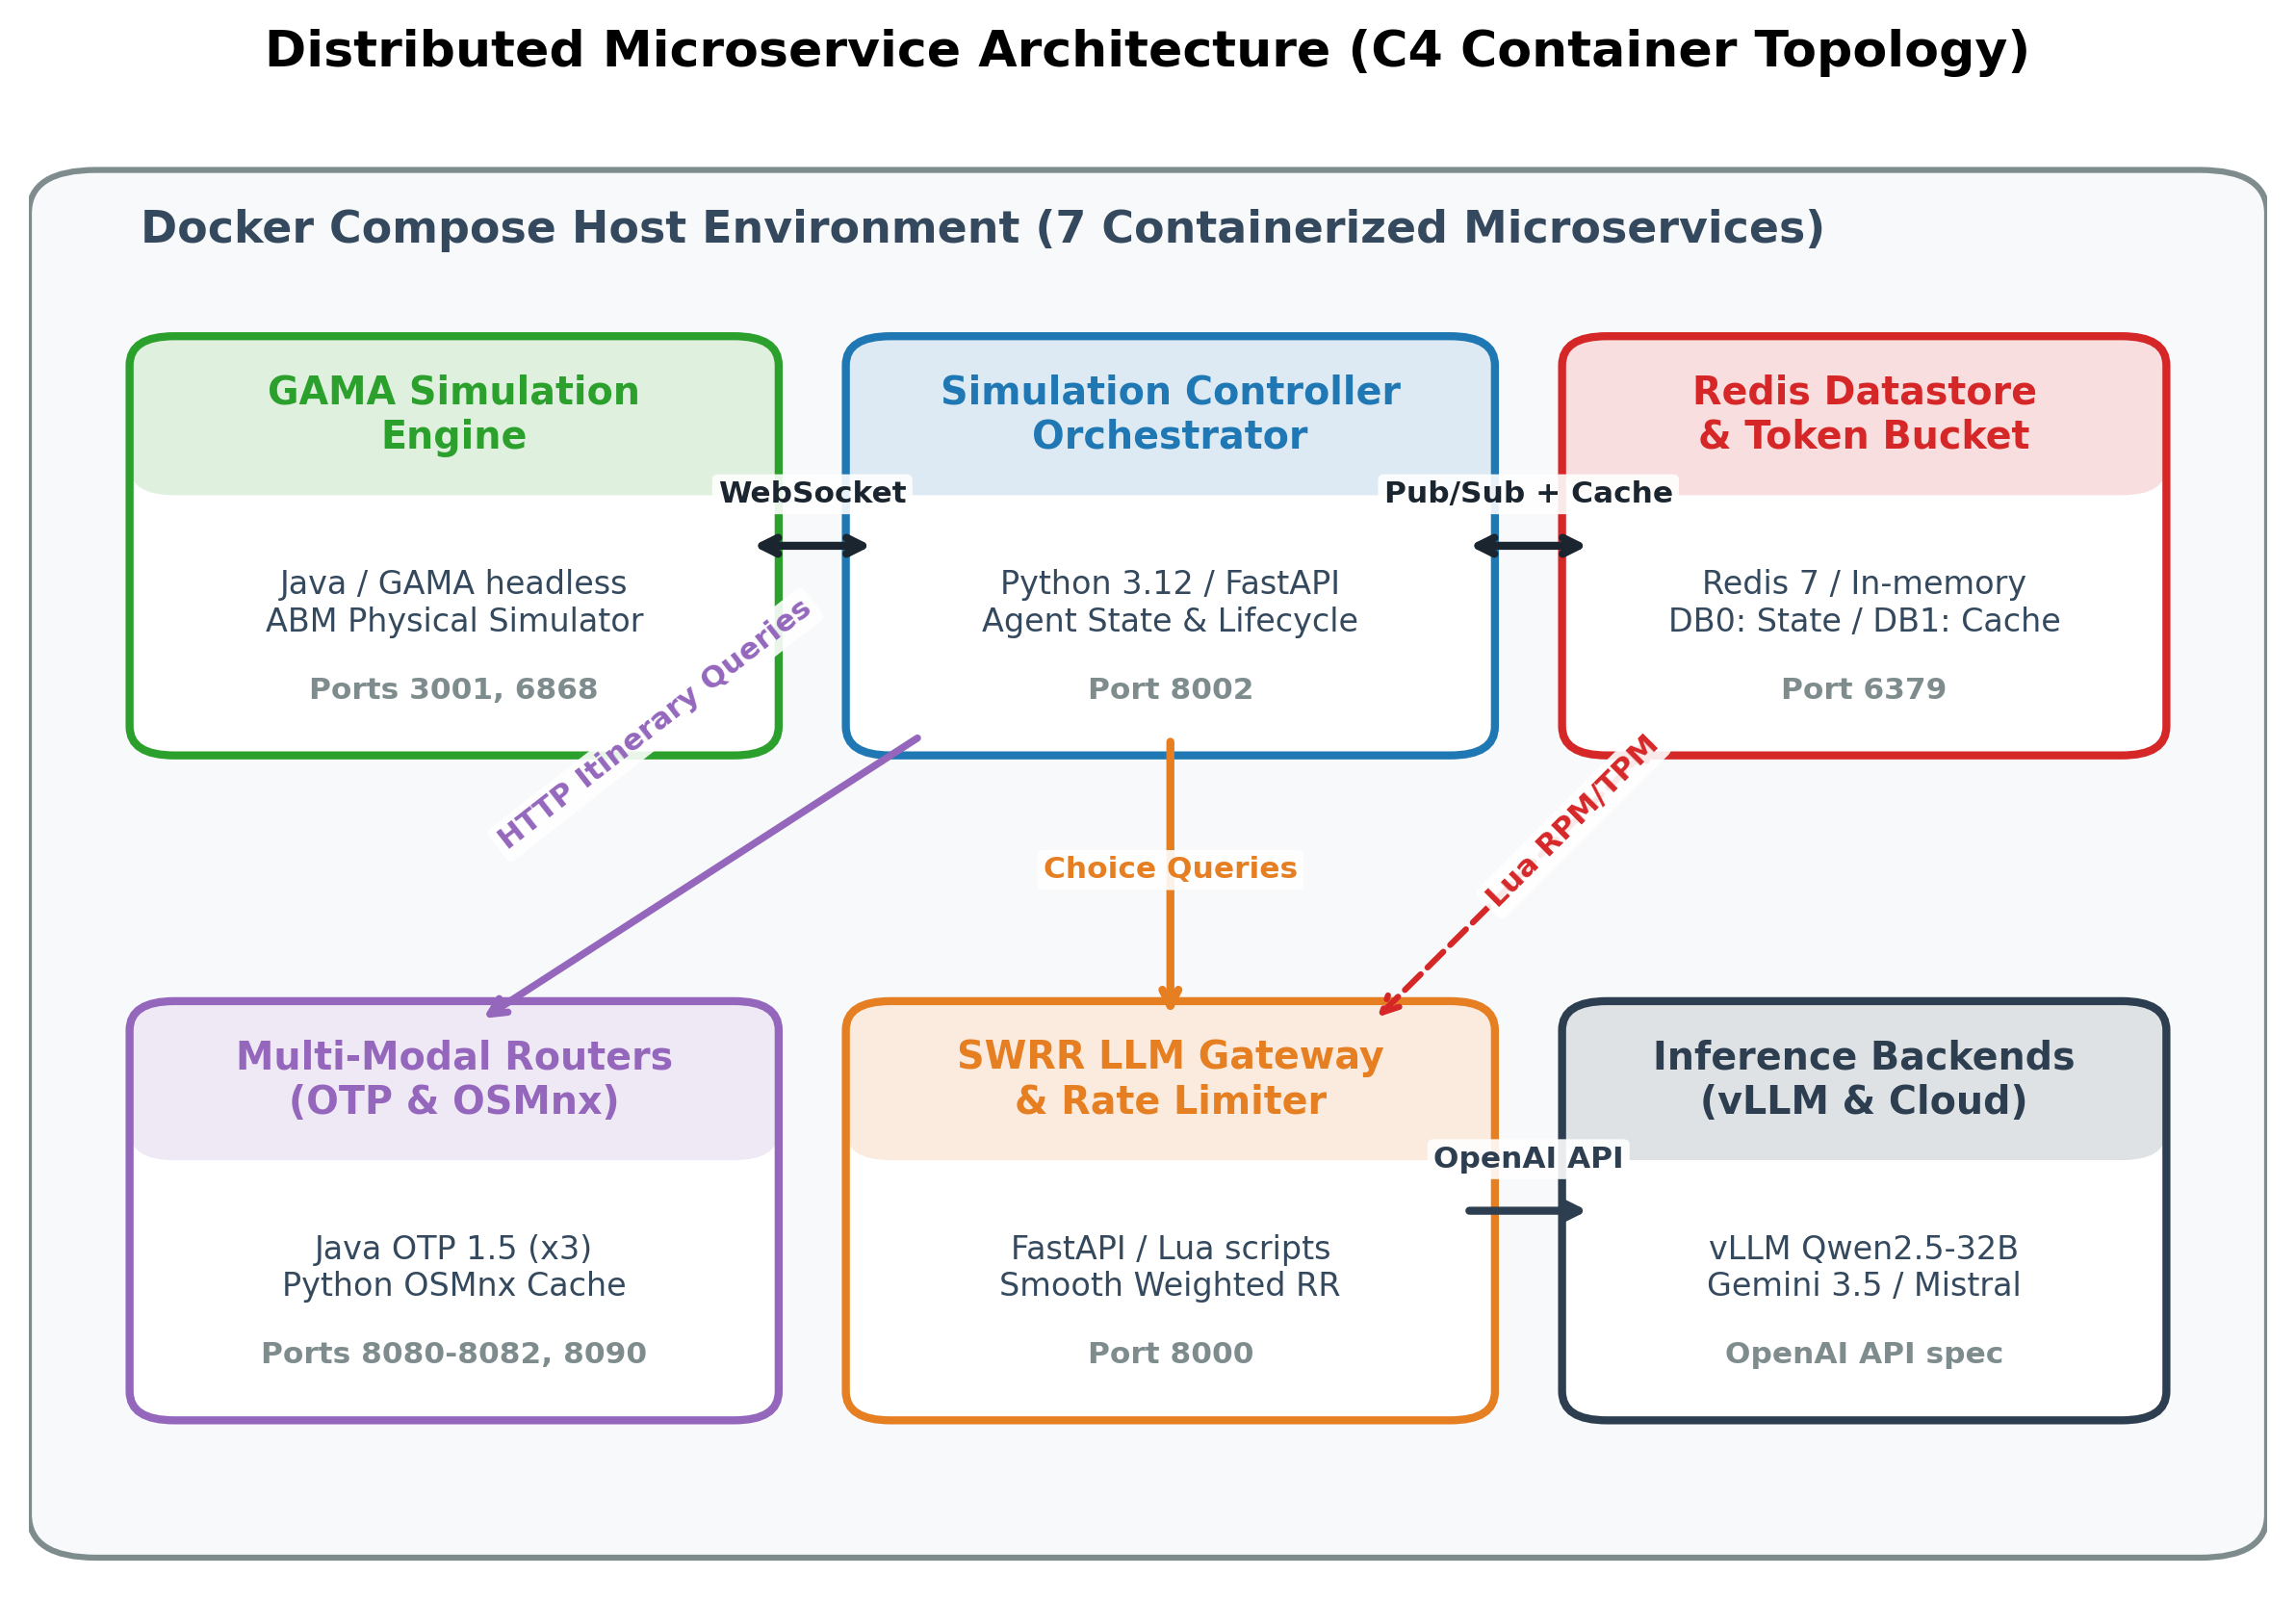
\includegraphics[width=0.90\textwidth]{images/fig_c4_container_topology}
\caption{Distributed container topology of the multi-agent simulation framework across seven microservices.}
\label{fig-c4_topology}
\end{figure*}

The simulation infrastructure coordinates seven containerized services managed through Docker Compose. Figure~\ref{fig-c4_topology} illustrates the container topology and communication channels.

The GAMA platform simulates continuous physical movement across the road and transit network. The FastAPI controller coordinates agent state transitions, triggers routing queries, and formats decision prompts. Redis acts as a high-throughput cache for candidate itineraries and pending decision requests.

\subsection{15.2 Decision Lifecycle UML Sequence}

Figure 15.2 illustrates the asynchronous message sequence governing each mobility decision.

\begin{Verbatim}
GAMA Server          Controller            Routers             ChromaDB          LLM / TypeSafe
    |                     |                   |                   |                     |
    |-- Agent IDLE ------>|                   |                   |                     |
    |   (event trigger)   |-- Route Request ->|                   |                     |
    |                     |   (OTP / OSMnx)   |                   |                     |
    |                     |<-- Candidates ----|                   |                     |
    |                     |                   |                   |                     |
    |                     |-- Filter Chains --+ (prune unavailable vehicles)            |
    |                     |-- Query Context --------------------->|                     |
    |                     |<-- Memories & Reflections ------------|                     |
    |                     |                                                             |
    |                     |-- Render Jinja2 / Choice Query ---------------------------->|
    |                     |   (sub-bullets, strict schema)                              |
    |                     |<-- Probability Vector & Justification ----------------------|
    |                     |                                                             |
    |                     |-- Multinomial Mode Draw (seed)                              |
    |<- Execute Move -----|                                                             |
    |   (WebSocket push)  |                                                             |
\end{Verbatim}

The controller initiates routing calculations as soon as an agent completes a previous activity. Vehicle chaining filters remove private modes if the vehicle remains parked elsewhere. Once the model returns a valid probability distribution, the controller executes a seeded multinomial draw.

\subsection{15.3 Asynchronous Backpressure and Simulation Synchronization}

Simulation clocks advance discrete simulation steps, whereas external language models exhibit variable network latency. Uncontrolled clock progression would cause agents to miss departure deadlines while awaiting API responses.

To maintain temporal synchronization, the controller implements a dual backpressure mechanism (\texttt{services/llm-agents/backpressure.py}).

First, a reactive backpressure function throttles GAMA \texttt{/sync} responses based on pending queue backlog. The interval formula specifies:
\[\Delta t = \text{cap} \cdot \left(\min\left(1, \frac{n}{N}\right)\right)^k\]
Parameter values are $k = 3.7$ and $\text{cap} = 30.0$ seconds. A floor threshold disables throttling when backlog remains below concurrency capacity.

\begin{figure}[h]
\centering
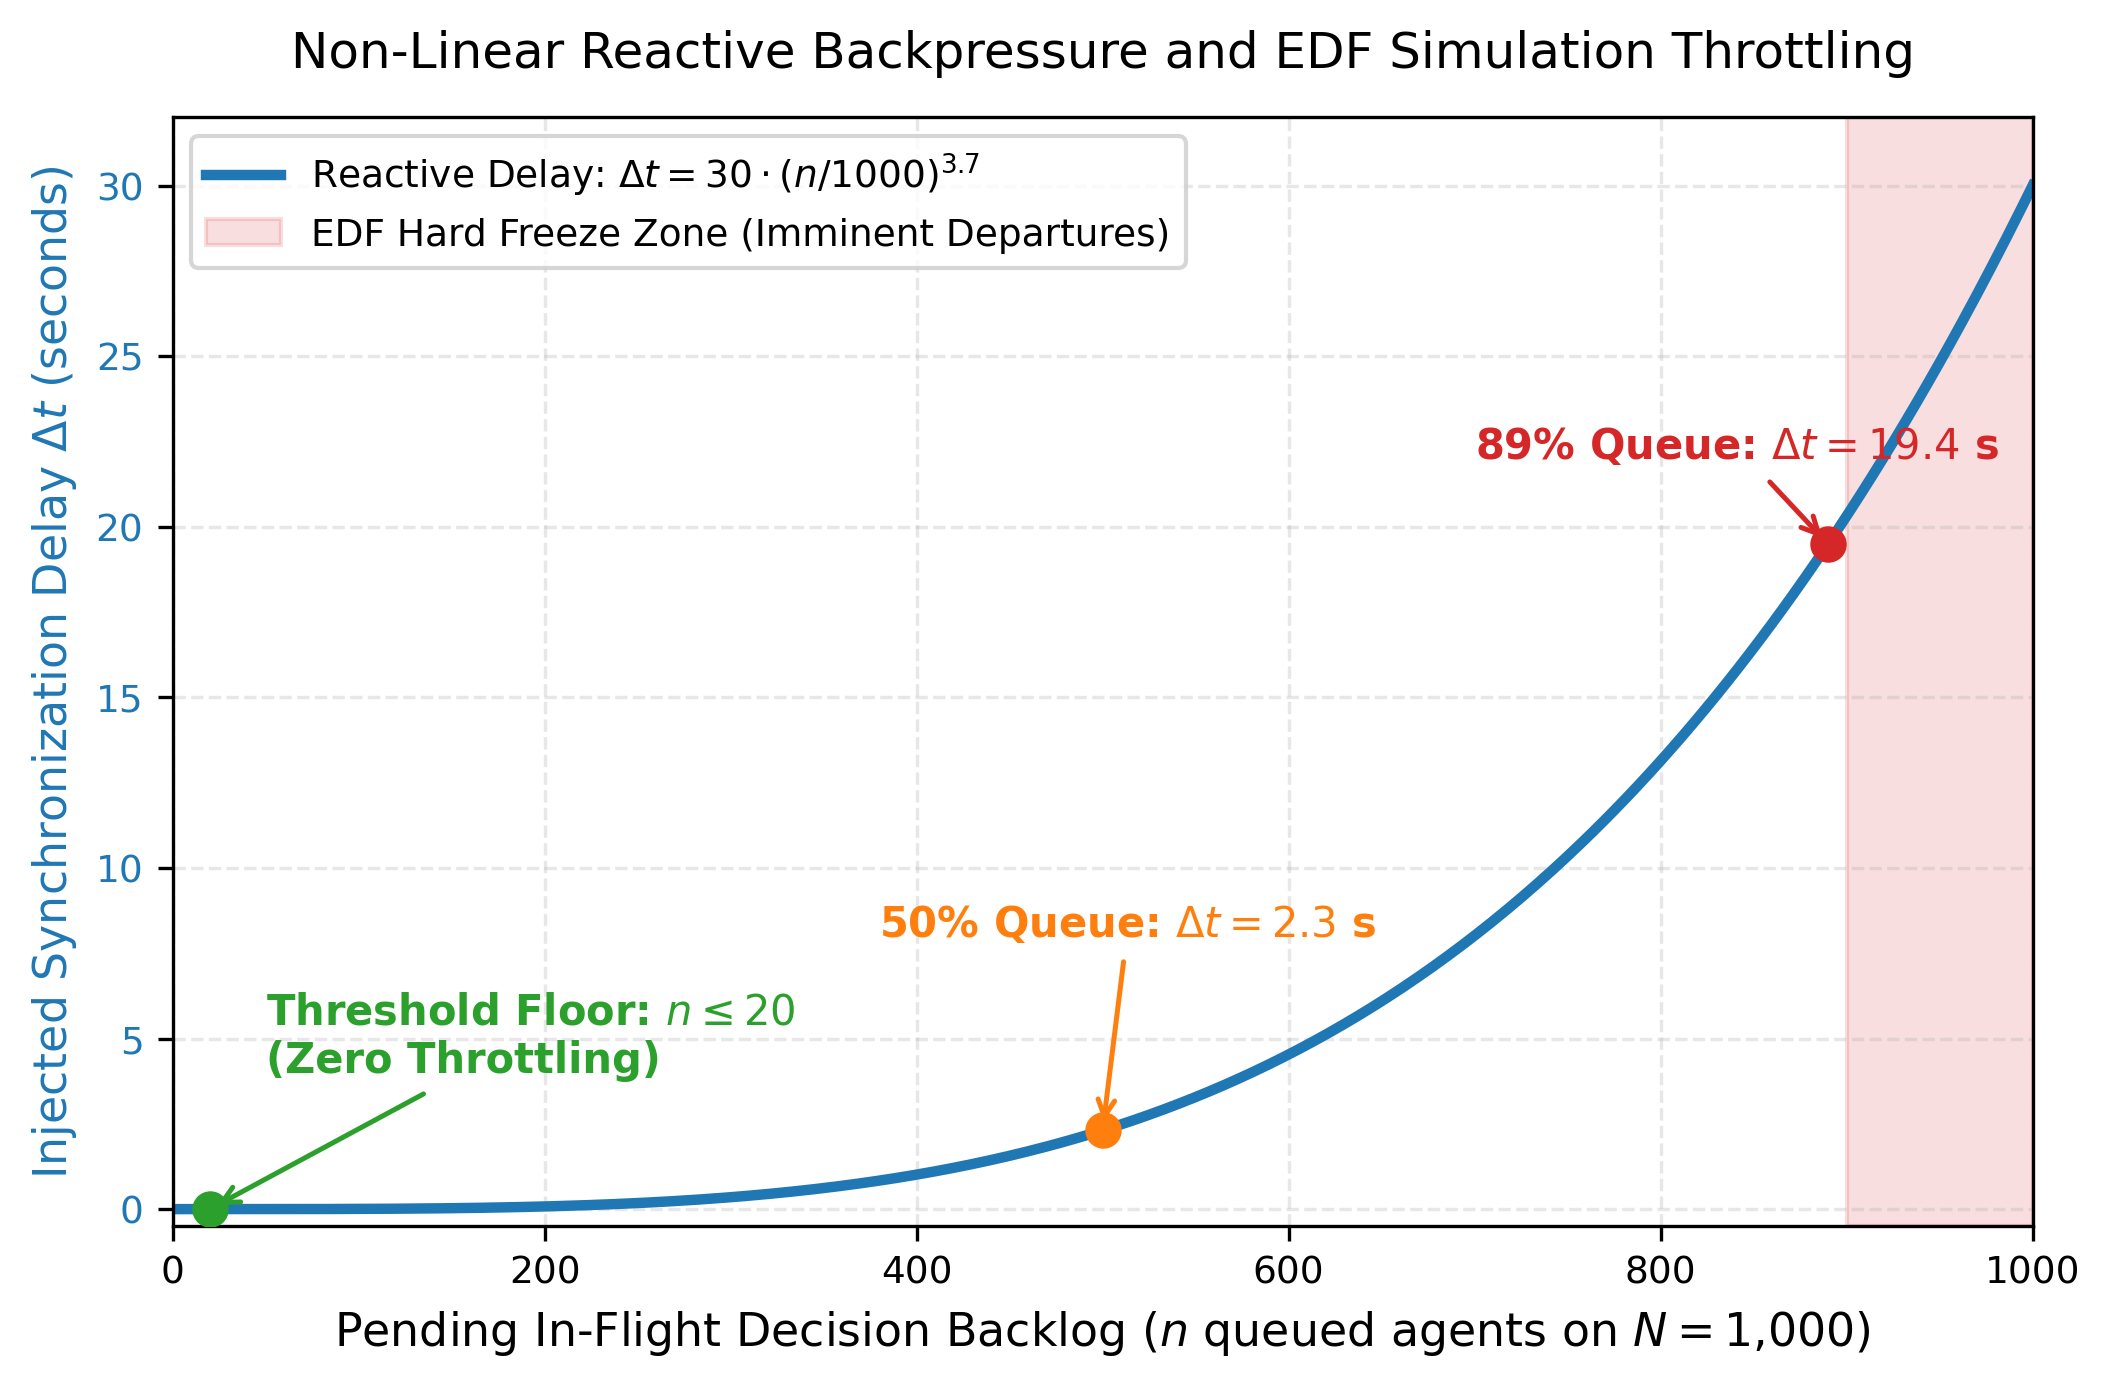
\includegraphics[width=0.90\columnwidth]{images/fig_backpressure_edf}
\caption{Reactive backpressure throttle curve ($k = 3.7$) and deterministic Earliest Deadline First (EDF) freeze threshold.}
\label{fig-backpressure}
\end{figure}

Second, an Earliest Deadline First (EDF) scheduler evaluates departure feasibility. If an agent faces an imminent departure whose decision remains in flight, the controller withholds the \texttt{/sync} confirmation. This pause holds simulation time until the decision resolves, preventing missed departures.

Figure~\ref{fig-backpressure} illustrates the non-linear reactive backpressure delay curve and the emergency EDF hold boundary.

\subsection{15.4 SWRR Gateway and Atomic Quota Reservation}

The inference gateway balances requests across multiple API keys using a Smooth Weighted Round-Robin (SWRR) algorithm.

To prevent HTTP 429 rate limit errors, Redis tracks token consumption using an atomic token bucket. An atomic Lua script checks both Requests-Per-Minute (RPM) and Tokens-Per-Minute (TPM) limits before granting execution tokens.

When executing scientific evaluation runs, the gateway activates the \texttt{force\_provider} flag. This setting disables automatic provider failover. If the target provider fails, the pipeline halts immediately, preventing uncontrolled cross-model contamination.

\subsection{15.5 TypeSafe Classifier Integration Engine}

The typed zero-shot classifier (\texttt{jev-1.13.0}) interfaces through \texttt{decideur\_typesafe.py}.

Unlike generative language models, the classifier accepts structured option sets as criteria rather than free text. The engine strips \texttt{[Output instructions]} from prompt templates because output types are enforced structurally:

\begin{Verbatim}
def instructions_servies(texte: str) -> str:
    coupe = texte.find("[Output instructions]")
    return (texte[:coupe] if coupe > 0 else texte).strip()
\end{Verbatim}

The classifier returns discrete option probabilities rounded to two decimal places. The engine enforces a strict sum tolerance:
\[\left|\sum_{i} p_i - 1.0\right| \le 0.02\]
The engine renormalizes weights when the probability sum falls within $[0.98, 1.02]$. If the sum deviates further, the engine marks the response as an invalid non-decision. The system logs non-decisions explicitly and excludes them from modal share calculations, rejecting silent default fallbacks.

\subsection{15.6 Sovereign vLLM Deployment and Hardware Parameters}

Researchers can execute all benchmarks locally using open-weight foundation models. Deploy the vLLM engine with the following command:

\begin{Verbatim}
vllm serve Qwen/Qwen2.5-32B-Instruct-AWQ \
  --quantization awq \
  --max-model-len 4096 \
  --gpu-memory-utilization 0.90 \
  --port 8000 \
  --seed 42
\end{Verbatim}

Serving \texttt{Qwen2.5-32B-Instruct-AWQ} requires a single GPU equipped with 24 GB of VRAM. Operating at temperature $\tau = 0.0$ and top-p 1.0 guarantees fully deterministic local replication.


\bibliographystyle{ACM-Reference-Format} 
\bibliography{sample}

\end{document}
